\documentclass[10pt, conference, letterpaper]{IEEEtran}
%\usepackage{showframe}
\usepackage{comment}
%\usepackage{showframe}
\setlength{\columnsep}{0.2 in}
%\usepackage[dvips]{epsfig}
%\usepackage{epstopdf}
%\usepackage[latin1]{inputenc}
%\usepackage[T1]{fontenc}


%\def\BibTeX{{\rm B\kern-.05em{\sc i\kern-.025em b}\kern-.08em
%    T\kern-.1667em\lower.7ex\hbox{E}\kern-.125emX}}

%\newtheorem{theorem}{Theorem}
%\setcounter{page}{1}

%\usepackage{graphicx,epstopdf}
%\epstopdfsetup{update}
%\DeclareGraphicsExtensions{.ps}
%\epstopdfDeclareGraphicsRule{.ps}{pdf}{.pdf}{ps2pdf -dEPSCrop -dNOSAFER #1 \OutputFile}


%\usepackage[margin=1.0in]{geometry}
%\usepackage{flushend}
%\usepackage{balance}
%\usepackage[dvips]{graphicx, color}

%\usepackage[dvips]{epsfig}
\usepackage[latin1]{inputenc}
\usepackage[T1]{fontenc}


\def\BibTeX{{\rm B\kern-.05em{\sc i\kern-.025em b}\kern-.08em
    T\kern-.1667em\lower.7ex\hbox{E}\kern-.125emX}}

\newtheorem{theorem}{Theorem}
%\setcounter{page}{1}

\usepackage{graphicx}
\usepackage{subfigure}
\usepackage{algorithm}
\usepackage{algorithmicx}
\usepackage{algpseudocode}
%\graphicspath{{./figures/}}
\usepackage{amsmath}
\usepackage{url}
\usepackage{array}
\usepackage{multirow}
%\usepackage[affil-it]{authblk}

\setlength{\columnsep}{0.2 in}
\begin{document}
\title{HashFlow  for Better Flow Record Collection}
%\author{Paper ID:xxx}
\author{Zongyi Zhao\IEEEauthorrefmark{1}, Xingang Shi\IEEEauthorrefmark{1}\IEEEauthorrefmark{4}, Xia Yin\IEEEauthorrefmark{1}, Zhiliang Wang\IEEEauthorrefmark{1}, Qing Li\IEEEauthorrefmark{2}\IEEEauthorrefmark{3}\\ zhaozong16@mails.tsinghua.edu.cn shixg@cernet.edu.cn \\
	yxia@tsinghua.edu.cn wzl@cernet.edu.cn liq8@sustc.edu.cn\\ 
	\IEEEauthorrefmark{1}Tsinghua University, \IEEEauthorrefmark{2}Southern University of Science and Technology\\ \IEEEauthorrefmark{3}PCL Research Center of Networks and Communications, Peng Cheng Laboratory, Shenzhen\\ \IEEEauthorrefmark{4}Corresponding Author}
%\affil[3]{Xingang Shi is the corresponding author.}
%\author{\IEEEauthorblockN{Zongyi Zhao\IEEEauthorrefmark{1}, Qing Li\IEEEauthorrefmark{2}, Mingwei Xu\IEEEauthorrefmark{1}, Lei Wang\IEEEauthorrefmark{2}, Meng Chen\IEEEauthorrefmark{1}}\\
%	\IEEEauthorblockA{\IEEEauthorrefmark{1}Department of Computer Science \& Technology, Tsinghua University\\
%		\IEEEauthorrefmark{2}Graduate School at Shenzhen, Tsinghua University}
%	\IEEEauthorblockA{zhaozy13@mails.tsinghua.edu.cn~li.qing@sz.tsinghua.edu.cn~xumw@tsinghua.edu.cn\\
%		lwang13@mails.tsinghua.edu.cn~chenm11@mails.tsinghua.edu.cn}}
\maketitle
\begin{abstract}
Collecting flow records is a common practice of network operators and researchers 
for monitoring, diagnosing and understanding a network. Traditional tools like 
NetFlow face great challenges when both the speed and the complexity of the network traffic increase. 
To keep pace up, we propose HashFlow, a tool for more efficient and accurate 
collection and analysis of flow records. The central idea of HashFlow is to  
maintain accurate records for elephant flows, but summarized records for mice flows, 
by applying a novel collision resolution and record promotion strategy to hash tables. 
We have implemented HashFlow as well as several latest flow measurement algorithms in a P4 software switch, and use traces from different operational networks to evaluate the algorithms.
In these experiments, for various types of traffic analysis applications, 
HashFlow consistently demonstrates a clearly better performance against 
its state-of-the-art competitors. 
For example, using a small memory of 1 MB, HashFlow can accurately record 
around 55K flows, which is often 12.5\% higher than the others.
For estimating the sizes of 50K flows, HashFlow achieves a relative error of around 11.6\%, 
while the estimation error of the best competitor is 42.9\% higher. 
It detects 96.1\% of the heavy hitters out of 250K flows with a size estimation error of 5.6\%, which is 11.3\% and 73.7\% better than  
the best competitor respectively.
At last, we show these merits of HashFlow come with almost no degradation of throughput.
\end{abstract}

\section{Introduction}
\label{section:introduction}
%The well functioning of computer networks depends on the efficient forwarding of packets as well as the effective management of networks. 
NetFlow\cite{claise_cisco_2004} is a widely used tool in network measurement and analysis.
It records traffic statistics in the form of flow records, where each record contains important 
information about a flow, for example, its source and destination IP addresses, 
start and end timestamps,  type of services, application ports, input and output ports, 
as well as the volume of packets or bytes, etc. 

A challenge in implementing NetFlow like tools is to keep up with the ultra high speed 
of network traffic, especially on high-bandwidth backbone links. For example, assuming an 
average packet size of 700 bytes, and a 40 Gbps link, the time budget for processing 
one packet is only around 50 nano-seconds\cite{zhang_more_2017}\cite{zhang_more_2015}\cite{wang_efficient_2019}.
 In an extreme case where packets of 40 bytes 
arrive at a speed of 100 Gbps, the time budget will be only a few nano-seconds. 
NetFlow also faces the high diversity of the traffic, where hundreds of thousands, 
even millions of concurrent flows appear in a measurement epoch. This pose stringent 
pressure on the scarce high-speed memories, such as on-chip SRAM with 1 $\sim$ 10 nano-seconds 
access delay\cite{li_flowradar:_2016}\cite{noauthor_access_nodate}.

One straightforward solution is to use sampling \cite{noauthor_sampled_nodate}, 
where out of several packets, only one of them gets processed and used to update the flow records.
However, sampling reduces processing overhead at the cost of fewer packets or flows being recorded, 
thus less accurate statistics that can be estimated. To remedy this, very enhanced sampling algorithms
\cite{hohn_inverting_2003}\cite{duffield_estimating_2005}\cite{tune_towards_2008}
have been proposed and tailored for specific measurement requirement, 
and their impact analyzed\cite{duffield2004}\cite{SamplingImpact}.
Another direction of solution is to use sketch (also referred as data streaming algorithms)
\cite{DataStreams2005}\cite{huang_sketchvisor:_2017}\cite{chen_counter_2017},
where a succinct data structure is designed and can be updated very efficiently. 
However, these sophisticated data structures and algorithms generally can only be used in limited scenarios, 
but not for the wide range of applications that the original NetFlow can support.

Towards accelerating flow record maintenance and achieving better statistics estimation, 
recently a few algorithms that make enhancement to a naive hash table and integrate sketches 
have been proposed, including OpenSketch\cite{yu_software_2013}, 
UnivMon\cite{liu_one_2016}, FlowRadar\cite{li_flowradar:_2016}, HashPipe\cite{sivaraman_heavy-hitter_2017},  
and ElasticSketch\cite{yang_elastic_2018}, etc. Both constant bound of the worst case delay and 
efficient utilization of memory are achieved, making them good candidates for general 
measurement applications in high-speed environment. 


%It allows the network operators to configure a parameter $N$ (e.g., $N=1000$). The network elements (switches or routers) will record a packet for every $N$ packets, and the estimated size of a flow is obtained by multiplying the recorded size of the flow by $N$. However, the method has several inherent shortcomings. Firstly, manually setting the sampling rate is hard for the network operators since it requires a deep understanding of the characteristics of the network traffic, and the current sampling rate may not be satisfiable and a better sampling rate is needed when network anomalies such as flooding attacks are present. Secondly, the small flows with only a small number of packets may be left out frequently, and flow size estimation for sampled flows often has large error. Finally, even if sampling is adopted in NetFlow, it remains to be an open question as how to access and update the flow records efficiently. Let's focus on the question of designing algorithms to allow efficient access and update of flow records since it is more fundamental than the configuration of sampling rate.


%Basically there are two challenges in designing the algorithms:

%\textbf{The time budget is small.} Note that nowadays the data rate in networks can be 40 Gbps or even 100 Gbps. Suppose the average packet size is 700 bytes (which is the average packet size of our trace files from campus networks as described in Section \ref{subsection:experimentsettings}), the processing time for a single packet may be as small as 56 ns. Notice that the network elements need to support many functions other than network measurement such as Layer 2/3 forwarding and ACLs which cost a substantial part of the time quotas, and a lot of ALU operations are necessary for the measurement function. Since the access time of on-chip SRAM is about 1-10 ns\cite{li_flowradar:_2016}\cite{noauthor_access_nodate}, only a few memory accesses are allowed to do the network measurement.

%\textbf{The memory budget is limited.} In a commercial data center (such as Facebook's data centers), each host may initiate 100s to 1000s concurrent flows\cite{roy_inside_2015}, so a ToR switch needs to handle 10K concurrent flows while a core switch needs to handle up to 100K flows concurrently.\footnote{$1K=10^3$ in this paper.} Suppose each flow record occupies 64 bytes of memory as recommended in \cite{cisco_configuring_2018} and SRAM is used to support high-speed forwarding. To accommodate 100K flow records at least 6.4MB of SRAM is needed. However, the size of available SRAM in the latest generation of switch ASICs is 50-100 MB only\cite{miao_silkroad:_2017}\cite{moshref_scream:_2015}, and other functions such as routing, scheduling and security need a substantial amount of SRAM.

%As sampling based NetFlow are widely used in today's networks, researchers have moved the focus to another direction recently, i.e., using hashing-based solutions to record the flow information, including sketches\cite{liu_one_2016}\cite{yu_software_2013} and flow arrays\cite{yang_elastic_2018}\cite{sivaraman_heavy-hitter_2017}. This type of methods has several advantages comparing with sampling methods. First of all, the time complexity for processing each packet is constant, which helps to provide predictability for the performance of network elements, and the memory requirement is limited. Moreover, when properly designed, the error rate of sketch is upper-bounded, and higher precision can be achieved.

%Theoretically, with unlimited time budget we can design a perfect algorithm (e.g., dichotomy) to access the flow records with no ancillary memory, or with unlimited memory budget we can design a perfect data structure (e.g., a perfect hash table) to access a flow record with only 1 memory access.

Following these efforts, we propose HashFlow, which makes a further step in squeezing memory consumption. 
The central idea of HashFlow is to  
maintain accurate records for elephant flows (i.e., flows with many packets), as well as summarized records for mice flows (i,e., flows with a few packets), 
by applying novel strategies of collision resolution and record promotion to hash tables. 
The collision resolution part eliminates collisions that may mix up packets 
from different flows, keeps a flow from being evicted until another flow with larger size collides with it, while fully utilizing the memory space by filling up nearly all hash table buckets.
On the other hand, the record promotion part allows the flows to grow in the summarized set, and bounces a flow back from the summarized set to the accurate set and replaces the original one which has smaller size when 
this flow becomes large enough. 
The performance bound can be analyzed with a probabilistic model, 
and with this strategy, HashFlow achieves a better utilization of space, 
and also more accurate flow records, without bringing extra complexity. 

We have implemented HashFlow, as well as several latest flow measurement algorithms mentioned above, 
including FlowRadar, HashPipe and ElasticSketch, in a P4-programmable \cite{bosshart_p4:_2014} software switch\cite{noauthor_bmv2:_2018}. To illustrate the implementability of HashFlow, we further implement it in a commodity P4 switch \cite{noauthor_barefoot_nodate} which has the type of Wedge 100BF-32X\cite{noauthor_edgecore_nodate}.
We then use traces from different operational networks to evaluate their effectiveness.
In these experiments, for various types of traffic analysis applications, 
HashFlow demonstrates a consistently better performance against 
its state-of-the-art competitors. 
For example, using a small memory of 1 MB, HashFlow can accurately record 
around 55K flows, which is often 12.5\% higher than the others.
For estimating the sizes of 50K flows, HashFlow achieves a relative error of around 11.6\%, 
while the estimation error of the best competitor is 42.9\% higher. 
It detects 96.1\% of the heavy hitters out of 250K flows with a size estimation error of 5.6\%, which is 11.3\% and 73.7\% better than  
the best competitor respectively.
At last, we show that these merits of HashFlow come with negligible degradation of throughput.

\iffalse
a solution based on hashing techniques for NetFlow in this paper, namely HashFlow. Our basic ideas in designing HashFlow are as follows:
\begin{itemize}
    \item Carefully sacrifice the time budget to improve the utilization of memory space by using multiple hash functions, so that we can accommodate more flow records at the expense of slightly more processing time.
    \item Record the elephant flows preferentially and drop the information about the mice flows when necessary to guarantee the accuracy of the recorded information since elephant flows are more important than mice flows for many applications such as heavy hitter detection and traffic engineering.
\end{itemize}

We implement HashFlow in P4\cite{bosshart_p4:_2014} and deploy it on bmv2\cite{noauthor_bmv2:_2018}. Our experimental results on bmv2 show that the average relative error of flow size estimation for heavy hitters is 36.5 times smaller, the average relative error of flow size estimation over all flows is 2.4 times smaller, and the precision for heavy hitter is improved by 19\% respectively, comparing to that of ElasticSketch\cite{yang_elastic_2018}, which is the state-of-the-art solution for network traffic measurement.
\fi

The remainder of the paper is organized as follows.
We introduce our motivation and central ideas in designing HashFlow in Section~\ref{section:background}. 
We present the algorithm details, as well as the theoretical analysis in Section~\ref{section:algorithmoverview}, and then present the implementation details in hardware P4 switch in Section~\ref{section:implementation}. 
Using real traffic traces, we analyze the parameters of HashFlow and compare it against other algorithms in Section~\ref{section:evaluation}.
% and discuss the related work in Section~\ref{section:relatedwork}. 
Finally we conclude the paper in Section~\ref{section:conclusion}.

\section{Background and Basic Ideas}
\label{section:background}
Formally, we define a flow record as a key-value pair $(key, count)$, 
where $key$ is the ID of the flow, and $count$ is the number of packets belonging to this flow. 
A simple example is like this: the flow ID contains the source and destination IP addresses, 
and packets with exactly the same source and destination belong to the same flow. 
The definition is general, since the flow ID can also be a subnet prefix, a transport layer port, 
or even a keyword embedded in application data. A naive method to maintain flow records is to 
save them in a hash table, but multiple flows may be hashed to the same bucket in the table. 
Mechanisms to resolve collisions in hash tables include classic ones like separate chaining 
and linear probing, and more sophisticated ones like Cuckoo hashing \cite{pagh_cuckoo_2004}.
However, in the worst case, they need unbounded time for insertion or lookup, thus are not 
adequate for our purpose. 

Before presenting HashFlow, we briefly review several recently proposed algorithms,
i.e., HashPipe\cite{sivaraman_heavy-hitter_2017}, ElasticSketch\cite{yang_elastic_2018} and FlowRadar\cite{li_flowradar:_2016}, and try to point out some minor defects in the algorithms. We will assume that the readers are familiar with the algorithms.

HashPipe\cite{sivaraman_heavy-hitter_2017} uses a series of independent hash tables (each with a different hash function). The first table is used to effectively accommodate new flows and evict the existing flows when collision occurs, otherwise new flows will have little chance to stay if large flows accumulate in the table. But on the other hand, this strategy frequently 
splits one flow record into multiple records that are stored in different hash tables, each with a partial count, 
since an existing flow may be evicted but new packets of this flow may still arrive later. 
This effect makes the utilization of memory less efficient, and makes the packet count less accurate. 

In ElasticSketch\cite{yang_elastic_2018}, due to the collisions and eviction strategy employed, a flow record may also be split 
into multiple records, and the packet counter is not accurate. The count-min sketch is introduced to help the flow size 
estimation. However, since the count-min sketch itself may not be accurate, the estimation accuracy is limited,  
which is especially true if the sketch is occupied by too many flows. 


%Unlike HashPipe and ElasticSketch, FlowRadar\cite{li_flowradar:_2016} tries to record all the flows. 
In FlowRadar\cite{li_flowradar:_2016}, flow information is encoded into a flow set, and then we can recover (some) flow IDs and the corresponding packet counts during the post processing phase. However, the chances that such decoding succeeds drop abruptly if the table is heavily loaded and there are not enough flows that don't collide with any other ones.

%FlowRadar records the size of every flow accurately when there is sufficient memory. However, when the value of $\frac{\text{num. of cells in the counting table}}{\text{num. of flows cached}}$ is less than some threshold (about 1.24), the performance of FlowRadar will degrade abruptly and many flows will fail to be decoded. So it is challenging to use it in the real networks where bursty traffic occurs frequently.

%As stated in Section~\ref{section:introduction}, there are two aspects that need to be considered when designing the measurement algorithms: (a) there is a small amount of SRAM (e.g., no more than 10 MB) in network elements that can be used for network measurement. (b) only a small amount of time (e.g., no more than 100 ns) are allowed for measurement algorithms to process a packet while the access time of SRAM is around 1-10 ns. So we aim to minimize the time/space complexity while guaranteeing the performance of the algorithm. First of all, we use hash table as a basic component of HashFlow. In the following we will present the reasoning behind the strategies we take in designing HashFlow.

With these in mind, we then analyze a few tradeoffs and design choices 
for time and space efficient collection of flow records.

1) {\em With limited memory, discard flows when necessary.} Pouring too many flows into a 
hash table or sketch will cause frequent collision, and either increase the processing overhead, 
or decrease the accuracy of the information that can be retrieved. 
For example, FlowRadar faces severe degradation in its decoding capability
 when the number of flows exceeds its capacity 
(this effect and the turning point can be clearly seen in our evaluation, 
for example, Fig. \ref{fig:comparison_concurrent_flows_increases_flow_monitoring} for flow set monitoring 
and Fig. \ref{fig:comparison_concurrent_flows_increases_fs_estimation} for flow size estimation).  
In most situations, network traffic is skewed such that 
only a small portion of elephant flows contain a large number of packets. 
For example, in one campus trace we use, 7.7\% of the flows contribute more than 85\% of the packets. 
It will be better to discard mice flows with few packets than elephant ones, 
since the latter have a greater impact on most applications, 
such as heavy hitter detection, traffic engineering and billing. It is often enough to maintain summarized information for the mice flows.

2) {\em A flow should be consistently stored in one record.} Both HashPipe and ElasticSketch 
may split one flow into multiple fragments stored in different tables. This not only wastes memory, 
but also causes the packet count less accurate, which in turn affects the eviction strategies.  
By storing a flow in a consistent record, we can achieve both better memory utilization and 
higher accuracy. 

3) {\em If better memory utilization can be achieved by trading off a little efficiency, have a try.} 
This is particularly worth to do when network equipment is becoming more ``software-defined'', 
where their functionalities can be  ``programmed'', 
and the additional operations can be easily paralleled or pipelined. 
By the nature of the ball and urn model \cite{urn} of hash tables, 
there will be a few empty buckets of a hash table that have never been used, and the utilization will be improved by feeding more flows into the hash table or hashing a flow multiple times to find a proper bucket. 
Both HashPipe and ElasticSketch propose to split the hash table into multiple small tables and use multiple hash functions to improve the utilization, 
but in different ways. Our collision resolution strategy is more similar to 
that of HashPipe than ElasticSketch. 
Later, we will show our strategy can make an effective use of the table buckets.

\iffalse
\subsection{It is impossible to store every flow with fixed memory.}
There are some sketches such as count-min sketch\cite{cormode_countmin_2005} and counter tree\cite{chen_counter_2017} that can pour any amount of information into it. These sketches are usually taken as a component to design some advanced measurement algorithms. For example, ElasticSketch\cite{yang_elastic_2018} takes a count-min sketch as the light table. The drawback of the type of sketches is that as the number of flows in the sketch increases, the error will be accumulated and the accuracy of the information provided by the sketches will degrade constantly. As an example, we create a count-min sketch with 4 rows and each row consists of 2K cells. We feed a number of flows into the sketch and then query the sketch for the sizes of the flows. Finally we calculate the ARE (Average Relative Error) of the estimated sizes of the flows as defined in Section~\ref{section:evaluation}. Fig.~\ref{fig:countminsketchare} shows that as the number of flows increases from 1K to 10K, the ARE of the estimated flow sizes is increased from 0.02 to 3.66. So if we feed too much information into the data structures like count-min sketch, the accuracy of the query result will be so low that it is nearly unusable. Take this in mind, we will discard the less important information to guarantee the accuracy of the most important information when designing HashFlow.

\begin{figure}
    \centering
    \begin{minipage}{0.24\textwidth}
        \centering
        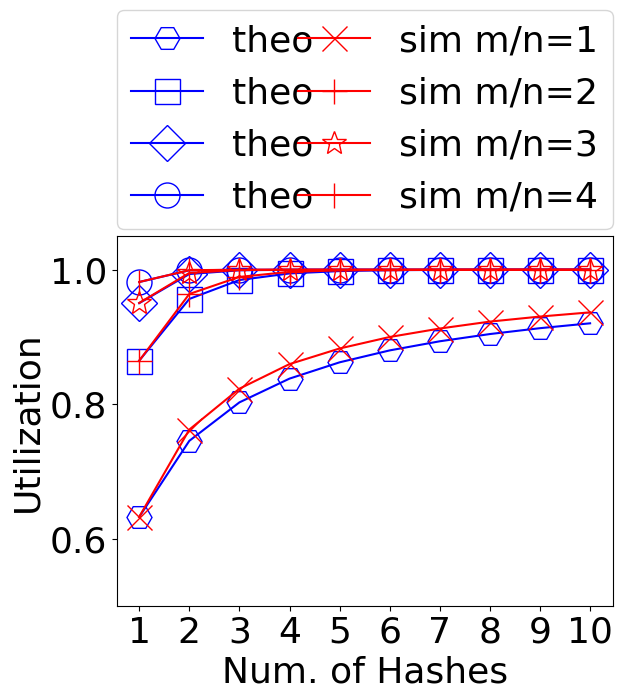
\includegraphics[width=\linewidth]{figures/exp84481/hash_table_utilization}
        \caption{The utilization ratio of the hash table when the number of hashes is increased from 1 to 10.}
        \label{fig:cachehitratio}
    \end{minipage}
    \begin{minipage}{0.24\textwidth}
        \centering
        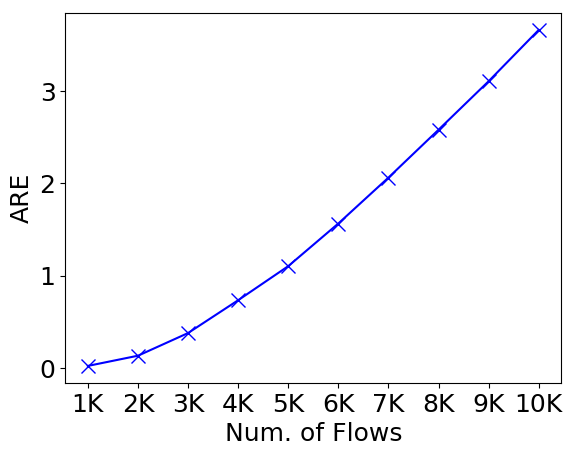
\includegraphics[width=\linewidth]{figures/exp84482/count_min_sketch_are}
        \caption{The average relative error of the count-min sketch as the number of flows increases from 1K to 10K.}
        \label{fig:countminsketchare}
    \end{minipage}
\end{figure}

\subsection{Elephant flows are more important than mice flows.}
Once the memory size is fixed, the number of flows that can be stored without degrading accuracy is fixed too. For most applications such as heavy hitter detection, traffic engineering and ISP billing, elephant flows are more important than small flows. On the contrary, usually it is enough to record the number of mice flows and the total number of packets corresponding to the flows. Moreover, due to the skewed characteristics of the network traffic\cite{benson_network_2010}, the number of mice flows is far greater than that of elephant flows, while the range of flow sizes of elephant flows is much greater than that of mice flows. For example, we define the flows with no less than 10 packets as elephant flows. For the CAIDA trace shown in Table~\ref{tab:netflowtraces},  only 3.1\% of the flows are elephant flows, the sizes of elephant flows have the range of [10, 110900], and 52.9\% of the packets are from the elephant flows. For the campus trace only 7.7\% of the flows are elephant flows while the sizes of elephant flows have the range of [10, 289877] and more than 85\% of the packets are from the elephant flows. So elephant flows are richer in information and it is reasonable to cache the elephant flows preferentially. 


\subsection{It is reasonable to tradeoff computation for higher memory utilization}
\label{subsection:computationmemoryutilizationtradeoff}
The conventional methods for handling collision in hash table such as cuckoo hash\cite{pagh_cuckoo_2004}\cite{chen_dynamic_2017} are infeasible for the scenario of network measurement since they require unlimited memory accesses in the worst case. Inspired by \emph{the power of two choices}\cite{byers_geometric_2004}\cite{doerr_stabilizing_2011}\cite{mitzenmacher_using_2007}\cite{mitzenmacher_power_2001}, we consider using multiple hash functions for handling collisions. When a new flow arrives we map it to the table using the first hash function. If collision occurs we map it using the second hash function. We do this all the way until an empty cell is found. If functions associated with the table are used up and no empty cell is found, the flow is discarded. 

Denote the number of hash functions associated with the table by $d$. Suppose the hash table consists of $n$ cells and we feed $n$ flows into it. The \emph{utilization} of the hash table is defined as $utilization=\frac{m}{n}$, where $m$ is the number of flows cached in the hash table successfully. 

In the case of $d=1$, after inserting $n$ flows, the probability that a given cell of the hash table is empty is 
\begin{equation}\label{key}
p_1 = (1 - \frac{1}{n})^n\approx \frac{1}{e}
\end{equation}

So the number of empty cells  as well as the number of flows that fail to be cached after insertion is $n\times p_1$. The utilization of the hash table is 
\begin{equation}
u_1 = \frac{n-n\times p_1}{n} = 1-p_1 = 1 - \frac{1}{e}
\end{equation}

Now consider the case where $d=2$. Firstly we map the flows to the table using the first function, which is the same as the case where $d=1$. So there will be $n\cdot p_1$ flows that are waiting to be cached using the second hash function. The probability that there is no flows mapped to a given cell during the second run of insertion is
\begin{equation}
(1 - \frac{1}{n})^{n\times p_1}\approx(\frac{1}{e})^{p_1}
\end{equation}

So the probability that a cell is empty after two runs of insertion is :
\begin{equation}
p_2 = p_1\cdot (\frac{1}{e})^{p_1}
\end{equation}
and the utilization of the hash table is:
\begin{equation}
u_2 = \frac{n - n\times p_2}{n} = 1 - p2
\end{equation}

Similarly, the utilization of the hash table when $d=k$ is:
\begin{equation}
u_k = 1 - p_k
\end{equation}
where $p_k$ is the probability that a given cell is empty after $k$ runs of insertion, and $p_1 = \frac{1}{e}$, $p_i = p_{i-1}\cdot (\frac{1}{e})^{p_{i-1}}$ for $i = 2, 3, \cdots, k$.

As shown in Fig.~\ref{fig:cachehitratio}, when we increase the value of $d$ from 1 to 10, the utilization of the hash table increases from 63\% to 92\%. So we can use more hash functions and improve the utilization of memory space by doing more computations.
\fi

\section{Algorithm Details}
\label{section:algorithmoverview}
In this section we explain how HashFlow works in detail, and present some theoretical analysis results, 
which are based on a probabilistic model.

\subsection{Data Structures and Algorithm}
The data structure of HashFlow is composed of a main table (${\mathbf M}$) and an ancillary table (${\mathbf A}$), 
each being an array of buckets, and each bucket (also called as cell) can store a flow record
in the form of \emph{(key, count)}, as mentioned in Section~\ref{section:background}. 
In the main table ${\mathbf M}$, flow ID will be used as \emph{key}, 
while in the ancillary table ${\mathbf A}$, a digest of flow ID will be used as \emph{key} to save the memory space.
We have a set of $d+1$ independent hash functions, i.e., $h_1, h_2, \cdots, h_d$, and $g$, 
where $d$ is a positive integer (we  call $d$ the  \emph{depth} of ${\mathbf M}$, and typically $d=3$). 
Each hash function $h_{i} (1 \le i \le d)$  randomly maps a flow ID to one bucket in ${\mathbf M}$, 
while $g$ maps the ID to one bucket in ${\mathbf A}$. 
A digest can be generated from the hashing result of the flow ID with any $h_i$.
When a packet arrives, HashFlow updates ${\mathbf M}$ and ${\mathbf A}$ with the following 
two strategies, as shown in Algorithm \ref{alg: process_packet}.

1) \textbf{Collision Resolution.} When a packet $p$ arrives, we first map it into the bucket indexed 
at $idx=h_1(p.\text{flow\_id})$ in the main table ${\mathbf M}$.  
If ${\mathbf M}[idx]$ is empty, we just put the flow ID and a count of 1 in the bucket (line 5$\sim$ 6).
If the bucket is already occupied by packets of this flow earlier, 
we just simply increment the count by 1 (line 7 $\sim$ 8). 
In either case, we have found a proper bucket for the packet, and the process finishes. 
If neither of the two cases happen, then a collision occurs, 
and we repeat the same process but with $h_2, h_3, \cdots, h_d$ one by one, 
until a proper bucket is found for the packet. 
This is a simple collision resolution procedure. 
Unlike HashPipe and ElasticSketch, it does not evict existing flow record from the main table, 
thus prevents a record from being split into multiple records. 

If collision cannot be resolved in the main table, 
then we try to record it in the ancillary table ${\mathbf A}$.
Here the action is more intrusive, 
as an existing flow will be replaced (discarded) if it collides with the new arrival (line 16 $\sim$ 19).

2) \textbf{Record Promotion.} If, in the ancillary table ${\mathbf A}$, $p$ succeeds to find the right bucket to reside, 
then it updates the packet count field of the record. 
Moreover, if the corresponding flow record keeps growing and the packet count becomes large enough, 
then we will promote the record by re-inserting it into the main table,
thus prevents large flows from being discarded. 
To implement this strategy, we keep in mind the sentinel flow record that has the smallest packet count 
among those records that collide with $p$ in the collision resolution procedure (line 9 $\sim$ 11). 
When a flow record in the ancillary table should be promoted, it will replace this sentinel  
we have kept in mind (line 22 $\sim$ 23).
We note that, instead of the flow ID, a shorter digest is used as keys in the ancillary table to 
reduce memory consumption. This may mix flows up, but with a small chance. When doing record promotion, we simply extract the flow ID from the current packet.


 
\begin{algorithm}[ht!]
    \caption{Update Algorithm of HashFlow on arrival of $p$}
    \label{alg: process_packet}
    \algrenewcommand\algorithmicwhile{\textbf{when}}
    \begin{algorithmic}[1]
        \State{//Collision Resolution}
        \State{$flowID \gets p.\text{flow\_id}, min \gets \infty, pos \gets -1$}
        \For{$i=1$ to $d$}
        \State{$idx\gets h_{i}(flowID)$}
        \If{${\mathbf M}[idx].key==NULL$}
        \State{${\mathbf M}[idx] \gets (flowID, 1)$}
        \Return
        \ElsIf {${\mathbf M}[idx].key == flowID$}
        \State{Increment ${\mathbf M}[idx].count$ by 1}
        \Return
        \ElsIf{${\mathbf M}[idx].count < min$}
        \State{$min \gets {\mathbf M}[idx].count$}
        \State{$pos \gets idx$}
        \EndIf
        \EndFor
        \State{$idx\gets g(flowID)$}
        \State{$digest \gets h_{1}(flowID)\%(2^{\text{digest width}})$}
        \If{${\mathbf A}[idx].count==0$ or ${\mathbf A}[idx].key \neq digest$}
        \State{${\mathbf A}[idx] \gets (digest, 1)$}
        \ElsIf{${\mathbf A}[idx].count < min$}
        \State{Increment ${\mathbf A}[idx].count$ by 1}
        \Else
        \State{//Record Promotion}
        \State{${\mathbf M}[pos].key \gets flowID$}
        \State{${\mathbf M}[pos].count \gets {\mathbf A}[idx].count+1$}
        \EndIf
    \end{algorithmic}
\end{algorithm}


We use a simple example with $d=2$ to illustrate the algorithm, as depicted in Fig. \ref{fig:datastructure}.
When a packet of flow $f_1$ arrives, $h_1$ maps it into an empty bucket indexed at $h_1(f_1)$, 
so the record becomes $(f_{1}, 1)$. 
When a packet of flow $f_2$ arrives, $h_1$ maps it into a bucket indexed at $h_1(f_2)$, 
where the record $(f_{2}, 5)$ has the same key, 
and the counter is simply incremented. 
When a  packet of flow $f_3$ arrives, it collides with the record $(f_4, 4)$ in the bucket indexed at $h_1(f_3)$. 
Then we try to resolve collision with $h_2$, but again, 
the packet collides with the record $(f_5, 10)$ in the bucket at $h_2(f_3)$. 
So we have to use $g$ to find a place in the ancillary table for the packet. 
Sadly, it collides again with the record $(f_6, 8)$, and we let it replace the existing one.
The last packet is from  flow $f_{7}$, and it goes through a similar process to that of $f_3$. 
The difference is that, at last, this packet finds its corresponding flow record of $(f_7,7)$ in the ancillary table, and after being updated the record appears to have greater packet count (i.e., 8) than the sentinel flow which has the packet count of 7. 
So we promote $(f_7, 8)$ by inserting it back into the main table, evicting the sentinel one. 
 


\begin{figure}[ht!]
    \centering
    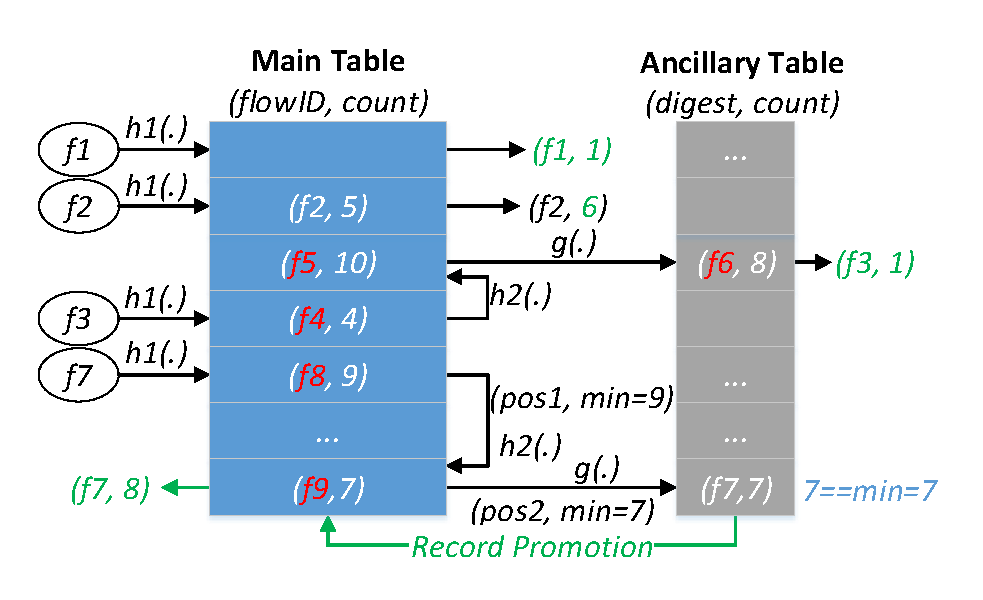
\includegraphics[width=\linewidth]{./figures/datastructure/datastructure.pdf}
    \caption{An example of HashFlow}
    \label{fig:datastructure}
\end{figure}


In Algorithm \ref{alg: process_packet}, we use multiple independent hash functions $h_i$$(i=1,2,\cdots,d)$ in a single main table ${\mathbf M}$.
Another choice is to use multiple small hash tables ${\mathbf M}_{i}$, each of which corresponds to an independent  hash function $h_{i}$. 
Algorithm \ref{alg: process_packet} can be modified straightforwardly: 
update the $i$-th small table ${\mathbf M}_{i}$ instead of ${\mathbf M}$ (line 5 $\sim$ 12),
remember which small table the sentinel record resides in (line 10 $\sim$ 11), 
and evict the sentinel record in the right small table (line 22 $\sim$ 23) to do record promotion.
In addition, we introduce a weight $\alpha (0<\alpha<1)$, 
such that the number of buckets in $\mathbf{M}_{i+1}$ is $\alpha$ times that in $\mathbf{M}_i$.

Readers may notice that HashPipe uses a similar scheme of pipelined tables, 
but there are a few important differences. 
First, HashFlow uses pipelined tables together with an ancillary table.
Second, the update strategy of these pipelined tables is different from that of HashPipe. 
Third,  our collision resolution procedure on the main table can be analyzed theoretically, 
based on which we can achieve a concrete performance guarantee on the number of accurate 
flow records that HashFlow can maintain.

\subsection{Analysis}
\label{analysis}
In the section, we propose a probabilistic framework that models the utilization of the  main table.
We first analyze the case where a multi-hash table is used for the main table,
then the case where pipelined tables are used. 
In either case, we assume that there are $m$ distinct flows fed into the main table, 
which has $n$ buckets in total, and uses $d$ hash functions.


%In the section we will analyze the utilization of a Main Table in the form of a normal hash table as well as a hierarchical hash table. Suppose the depth of a hash table is $d$, i.e., there are $d$ hash functions associated with it. It consists of $n$ cells and there are $m$ distinct flows feed into it. The \emph{utilization} is defined as $utilization=\frac{n'}{n}$, where $n'$ is the number of flows cached successfully. 

\textbf{Multi-hash table.} First, consider the case when $d=1$, 
where the analysis follows a classic ball and urn problem\cite{urn}.
After inserting $m_1=m$ flows randomly into $n$ buckets, 
the probability that a given bucket is empty is 
\[\label{equation1}
p_1 = (1 - \frac{1}{n})^{m_1} \approx e^{-\frac{m_1}{n}},
\]
and the utilization of the table is 
$u_{1}=1-p_{1}= 1 - e^{-\frac{m_1}{n}}.$
Since each bucket can contain only one flow record due to our collision resolution strategy, 
the number of flows that fail to be cached in $\mathbf{M}$ after this round is $m_1-n\times(1-p_1)$.

Now consider the case of $d=2$. 
Essentially, a flow tries another bucket with $h_2$ if it finds out 
that the first bucket it tries has already been occupied. 
Since we don't care which exact flow is stored in the table, 
we slightly change the update process to the following one.
We take two rounds. In the first round, 
we feed all the $m_1$ flows into the table with $h_1$, exactly the same as $d=1$.
In the second round, we feed all the remaining flows that have not been kept in $\mathbf{M}$ into the table again, 
but this time with $h_2$. 
Assume $\mathbf{M}$ is empty before the second round starts, 
then after the $m_2=m_1-n\times(1-p_1)$ flows left by the first round have been inserted in the second round, 
a bucket will be empty with probability $e^{-\frac{m_2}{n}}$. 
However, $\mathbf{M}$ is actually not empty before the second round, 
and at that time a bucket in it is empty with probability $p_1$.
Since $h_1$ and $h_2$ are independent, we know after the second round, 
the probability that a bucket is still empty becomes $p_2 \approx p_1 \times e^{-\frac{m_2}{n}}$, 
and the number of flows that have not been inserted into $\mathbf{M}$ will be $m_3=m_1-n\times(1-p_2)$.
The utilization of $\mathbf{M}$ now becomes $u_2=1-p_2$.

The analysis for the slightly changed process can be extended to cases when $d>2$. 
In the $k$-th round, $m_k$ flows are fed into a hash table with a new hash function $h_k$, 
where there are already $n \times (1-p_{k-1})$ buckets being occupied in the previous rounds. 
Then after the $k$-th round, the probability that a bucket is empty is
\begin{eqnarray}
\label{xx1}
p_k & \approx &p_{k-1} \times e^{-\frac{m_k}{n}} \nonumber \\
& = & p_{k-1} \times e^{-\frac{m_1-n \times (1-p_{k-1})}{n}} \nonumber \\
& = & p_{k-1} \times e^{1-\frac{m_1}{n}-p_{k-1}} \nonumber \\
& = & p_{k-1} \times e^{1-\frac{m}{n}-p_{k-1}}
\end{eqnarray}
for $k \ge 2$. With Equation (\ref{xx1}), for any given $d$, $m$, and $n$, 
we can recursively compute the probability $p_d$ that a bucket is empty in the hash table after $d$ rounds. 
Then the utilization of the hash table will be $1-p_d$. 
We note that there is a slight difference between this model and our multi-hash table, as will be shown later.

\iffalse
In the case of $d=k, k\ge 2$, suppose the probability that a given cell is empty after the first $k-1$ runs of insertion is $p_{k-1}$. The number of flows that are waiting to be cached using the $k^{th}$ hash function is $m - n(1-p_{k-1})$, so the probability that there is no flow mapped to a given cell during this run of insertion is
\begin{equation}\label{equation3}
(1 - \frac{1}{n})^{m - n(1- p_{k-1})}\approx (\frac{1}{e})^{p_{k-1}}\cdot(\frac{1}{e})^{(\frac{m}{n} - 1)}
\end{equation}

And the probability that a cell is empty after $k$ runs of insertion is :
\begin{equation}\label{equation4}
p_k = p_{k-1}\cdot (\frac{1}{e})^{p_{k-1}}\cdot(\frac{1}{e})^{(\frac{m}{n} - 1)}
\end{equation}
and the utilization of the hash table is:
\begin{equation}\label{equation5}
u_k = \frac{n - n\times p_k}{n} = 1 - p_k
\end{equation}
\fi



\begin{figure*}[t]
    \centering
    \mbox{
        \subfigure[Multi-hash Table\label{multihash}]{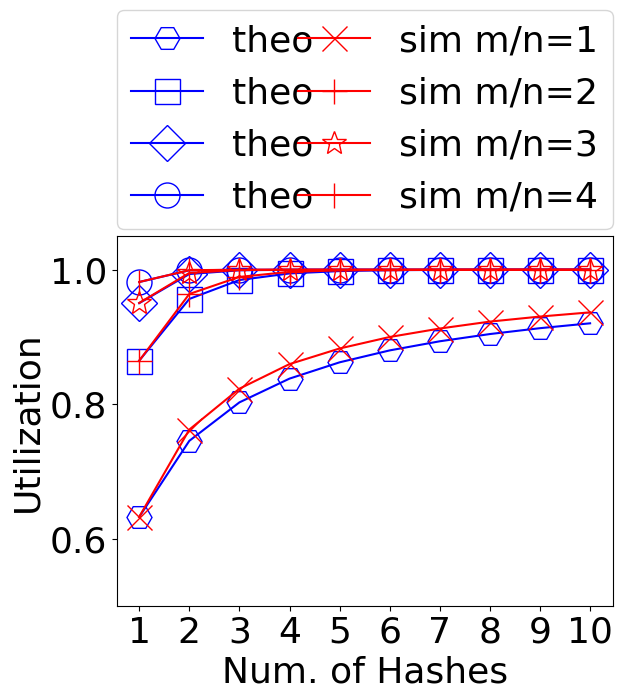
\includegraphics[width=0.24\linewidth]{figures/exp84481/hash_table_utilization}}
        \subfigure[Pipelined Tables\label{pipeline1}]{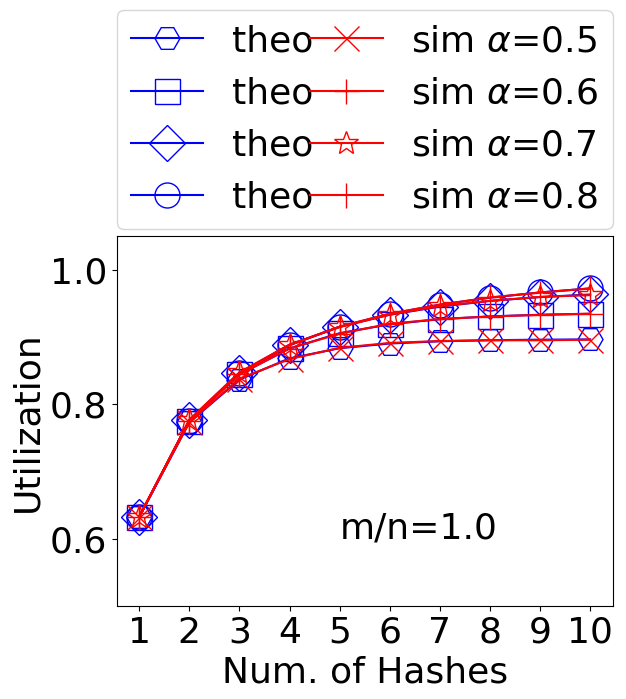
\includegraphics[width=0.24\linewidth]{figures/exp84489/pipelined_tables_utilization_ratio_10}}
        \subfigure[Pipelined Tables\label{pipeline2}]{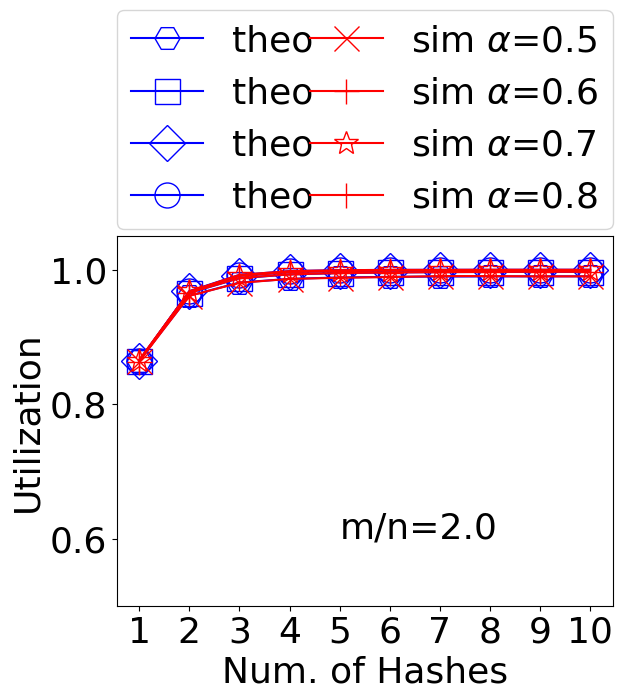
\includegraphics[width=0.24\linewidth]{figures/exp84489/pipelined_tables_utilization_ratio_20}}
        \subfigure[Improvement on Utilization\label{improvement}]{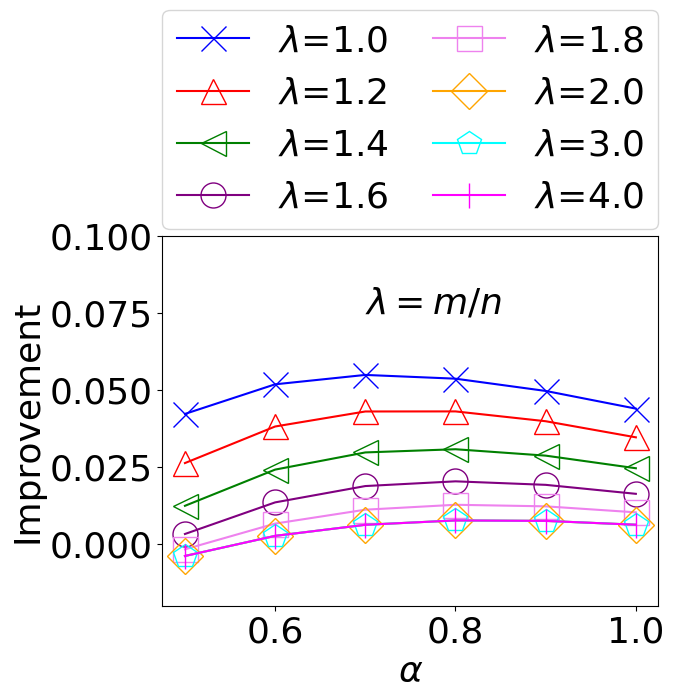
\includegraphics[width=0.24\linewidth]{figures/exp84488/improvement}}
    }
    \caption{Utilization of the multi-hash table and the pipelined tables}
    \label{fig:pipelinedtablesutilizationratio}
\end{figure*}

\textbf{Pipelined tables.}
Let $n_k$ be the number of buckets in the $k$-th table $\mathbf{M}_k$ such that $n_{k+1}=\alpha \times n_k$, 
where $\alpha$ is the  pipeline weight.
We perform a similar modification to our collision resolution procedure with pipelined tables, 
such that in the $k$-th round, 
all packets goes though the $k$-th table before they are fed into the $k+1$-th table in the $k+1$-th round.
We use the same notations $p_k$, $m_k$ and $u_k$ as those in the first model.
Since $\sum_{k=1}^dn_k=\sum_{k=1}^d(\alpha^{k-1} \times n_1)=\frac{1-\alpha^{d}}{1-\alpha} \times n_1$, 
we get $n_1=\frac{1-\alpha}{1-\alpha^{d}} \times n$, 
and $n_k=\alpha^{k-1} \times \frac{1-\alpha}{1-\alpha^{d}} \times n$.

The first round works exactly the same as that in the previous model, 
so we get $p_{1}=(1 - \frac{1}{n_1})^{m_1} \approx e^{-\frac{m_1}{n_{1}}}$, 
$u_1=1-p_1$, and $m_2=m_1-n_{1}\times(1-p_1)$.

For the $k$-th round, we know $m_k$ flows are to be fed into the table $\mathbf{M}_{k}$ with $n_k$ buckets, 
so we get $p_{k} \approx e^{-\frac{m_k}{n_{k}}}$, 
and the number of flows left after this round is 
\begin{equation}
\label{xxx1}
m_{k+1}  =  m_{k}-n_{k}\times(1-p_k). 
\end{equation}
Dividing  both sides of Equation (\ref{xxx1}) by $n_{k+1}$, we get 
\begin{eqnarray}
\frac{m_{k+1}}{n_{k+1}} & = & \frac{n_k}{n_{k+1}}  \times \frac{m_{k}-n_{k}\times(1-p_k)}{n_k} \nonumber \\
& = & \alpha^{-1} \times \left( \frac{m_k}{n_k} - 1 + p_k  \right), \nonumber
\end{eqnarray}
which is just
\begin{equation}
\label{xxx2}
-\ln p_{k+1}=\alpha^{-1} \times (-\ln p_k -1 + p_k).
\end{equation}

From Equation (\ref{xxx2}), we finally get 
\begin{equation}
\label{xxx3}
p_{k+1}=(p_k)^{\frac{1}{\alpha}} \times e^{\frac{1-p_k}{\alpha}}. 
\end{equation}

With Equation (\ref{xxx3}), for any given $d$, $m$, and $n$, 
we can recursively compute the probability $p_k (1 \le k \le d)$ that a bucket is empty in the $k$-th hash table.
Then the utilization of the pipelined tables will be 
\begin{equation}
\label{pipelineutil}
\frac{\sum_{k=1}^{d} (n_k \times (1-p_k))}{\sum_{k=1}^{d} n_k} = 1- \frac{1-\alpha}{1-\alpha^{d}} \times \sum_{k=1}^{d}(\alpha^{k-1} \times p_{k}).
\end{equation}

\iffalse
$m_i$ is the number of flows that arrives at this table. Thus we have
\begin{IEEEeqnarray}{crc} 
n = \sum_{i =1}^d n_i = \sum_{i =1}^d \alpha^{i-1}n_1\\
m = m_1
\end{IEEEeqnarray}

We denote $\sum_{i =1}^d \alpha^{i-1}$ by $\delta$. For the first table, after inserting $m_1 = m$ flows, the probability that a given cell is empty is
\begin{IEEEeqnarray*}{crc}
    p_1 = (1 - \frac{1}{n_1})^{m_1}\approx (\frac{1}{e})^{\frac{m_1}{n_1}} = (\frac{1}{e})^{\delta\cdot\frac{m}{n}}
\end{IEEEeqnarray*}

For the $k^{th}$ table ($k= 2, \cdots, d$), after inserting $m_k$ flows, the probability that a given cell is empty is 
\begin{equation}
p_k = (1 - \frac{1}{n_k})^{m_k} \approx (\frac{1}{e})^{\frac{m_k}{n_k}}
\end{equation}

Notice $m_k = m_{k - 1} - n_{k - 1}(1 - p_{k - 1})$, we get
\begin{IEEEeqnarray*}{crc}
    \frac{m_k}{n_k} &=& \frac{m_{k - 1} - n_{k - 1}(1 - p_{k - 1})}{\alpha\cdot n_{k-1}} \\
    &=& \frac{1}{\alpha}(p_{k - 1} - \ln p_{k - 1} - 1)
\end{IEEEeqnarray*}

So $p_k$ corresponding to each sub-table can be given by
\begin{IEEEeqnarray*}{crc}
    p_k = e^{\frac{1}{\alpha}(1-p_{k-1})}(p_{k-1})^{\frac{1}{\alpha}}
\end{IEEEeqnarray*}

The utilization of the tables is 
\begin{IEEEeqnarray*}{crc}
    utilization &=& 1  - \frac{1}{n}\sum_{i = 1}^{d}n_kp_k
    = 1 - \frac{1}{\delta}\sum_{i = 1}^{d}\alpha^{i - 1}p_i
\end{IEEEeqnarray*}
\fi

Now we will show how accurate the models are. 
In Fig. \ref{multihash},
we use $n=$100K buckets, with different depth $d$ from 1 to 10, 
and vary the traffic load $m/n$ from 1 to 4. As can be seen there, 
when $m/n \ge 2$, the multi-hash table model provides nearly perfect predictions.

In Fig. \ref{pipeline1} and Fig. \ref{pipeline2}, we use a similar setting as above, with $n=$100K and $d$ from 1 to 10,
but we vary the pipeline weight $\alpha$ between 0.5 to 0.8. 
This time the model and the simulation results match quite well, 
since  arranging the packet arrivals in rounds, as we have done in the model,  
actually does not affect the final probability (we omit the proof due to space limitations).

With these two models, we can predict the utilization of our main table, 
as long as the traffic load $m/n$ is known.
We can see that more hash functions will improve the utilization.
In the case of $m/n=1$, the utilization  increases from 63\% to 83\% 
when $d$ is increased from 1 to 3, and from 83\% to 92\% when $d$ is increased from 3 to 10.
As more hash functions require more hash operations and memory accesses in the worst case, 3 hash functions seems to be a  sweet spot, and we use $d=3$ by default in our evaluations.

Fig. \ref{improvement} shows, when $d=3$, 
pipelined tables always improves the utilization upon  multi-hash table, regardless of the traffic load.
As shown there, when $\alpha=0.7$ and $m/n=1$, up to 5.5\% more utilization can be achieved.
Our evaluation will adopt the pipelined scheme, where $\alpha=0.7$ seems to be the best choice.

%. For example, $H$ is a hash table with 100K cells and there are 3 hash functions, i.e., $h_1$, $h_2$ and $h_3$, associated with it. The hash functions can map a flow ID to the hash table independently and randomly. We refer to this hash table as \emph{normal} hash table. We reconstruct the hash table such that the hash table consists of 3 sub-tables and $h_1$, $h_2$ and $h_3$ are associated with the sub-tables respectively. The sizes of the sub-tables are determined by a  \emph{hierarchy coefficient} $\alpha$ ($0 < \alpha <= 1$) such that $S_i = \alpha\times S_{i-1}$ for $i = 2, 3$ where $S_i (i = 1, 2, 3)$ is the size of sub-table $i$. We feed 100K randomly generated flow IDs into the normal hash table as well as hierarchical hash tables with various $\alpha$ and then calculate the utilization of the hash tables. Fig.~\ref{fig:simulator_hierarchical_hashtable_performance} shows that the utilization of hierarchical hash tables are better than that of a normal hash table when the value of $\alpha$ is no less than 0.5. Since the MT of HashFlow is a hash table essentially, the utilization of MT should be higher if it is organized hierarchically and the hierarchy coefficient is set properly. 
%\begin{figure}
%    \centering
%    \begin{minipage}{0.24\textwidth}
%    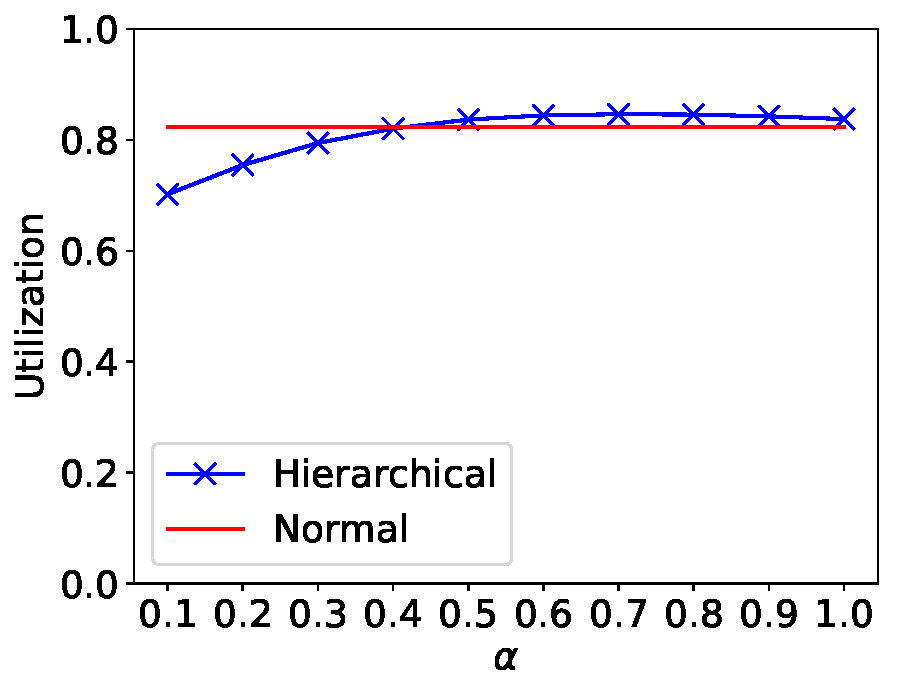
\includegraphics[width=\linewidth]{figures/exp84483/hash_table_utilization}
%    \caption{The utilization of a normal hash table as well as that of a hierarchical hash table as the value of $\alpha$ increases from 0.1 to 1.0.}
%    \label{fig:simulator_hierarchical_hashtable_performance}
%    \end{minipage}
%\end{figure}


\section{Implementation in P4 Hardware Switch}
\label{section:implementation}
As stated before, we have implemented HashFlow in bmv2, the software P4 switch, as well as in a hardware P4 switch which has the type of Wedge 100BF-32X\cite{noauthor_edgecore_nodate}. The code can be found at \cite{zhao_hashflow_2018}. Although both versions of the algorithm are implemented using P4$_{14}$, the grammar checking of the hardware switch is stricter than that of the software switch, and the implementation is heavily limited by the resource restrictions of the hardware. In this section, we will discuss the hardware implementation of HashFlow in detail.

The P4 program will be compiled into a pipeline, which consists of multiple stages. Multiple small match-action tables can be packed into a stage, and a large table may span multiple stages. The tables within the same stage can be executed in parallel, while the stages can only be executed serially and tables that are dependent on each other must be distributed among different stages. The compiler will analyze the dependency relationship of the tables and arrange the tables within the stages automatically. The amount of processing within a single stage is upper bounded, so the processing time of a single stage is limited. Moreover, to upper bound the processing delay within a single P4 switch, the number of stages that a switch can support is limited. Our switch can support 12 stages at most.
In our implementation, we identify a flow with the typical 5 tuples and store the flow records into 6 register arrays, i.e., one register array for source/destination IP address, protocol, source/destination port and packet count respectively. A register array can only be accessed using stateful ALUs, which can execute a simple program atomically. As an action of P4 cannot access more than one register array (through stateful ALUs), we implement 6 match-action tables to access a flow record. Since accesses of the IP addresses, protocol and ports are independent, and the operations imposed upon packet count are determined by the result from accessing the flow ID, the tables corresponding to the arrays of IP addresses, protocol and ports can be packed into a single stage, while the table corresponding to the packet count has to be put into another stage. We define an \emph{iteration} to be all the processing operations corresponding to a pipelined table or the ancillary table, so HashFlow contains $d+1$ iterations. In our implementation, the first iteration needs 2 stages, and each of the following iterations needs 4 stages, so HashFlow needs $4\times d + 2$ stages and only $d\le 2$ is allowed in our P4 switch. To support more pipelined tables, more resources or advanced techniques to refine the implementation are needed.

To allow the pipelining of the packets, multiple tables sharing the same register array in a pipeline can only access the resource exclusively, which means that only one table can access the resource when processing a packet. In Algorithm~\ref{alg: process_packet}, we may have to visit the hash table $d$ times when doing collision resolution, violating the access restriction. We can address the problem by splitting the hash table into $d$ small tables, so only the pipelined-tables scheme of main table is feasible in P4 hardware switch. However, when computing the index from a flow ID, the size of the index space must be the power of 2, so the table arrangement stated in Section~\ref{analysis}, i.e., decreasing the size of the pipelined tables in a factor of 0.7, is infeasible. We simply set the size of each table to be the same in our hardware implementation.

Another challenge in implementing HashFlow is that record promotion requires to revisit one of the pipelined tables, even if we have visited every table when doing collision resolution, thus violating the access restriction. Our solution is to resubmit the current packet and process it again when doing record promotion. By marking some metadata, we will be able to evict an existing flow record and set up a new record for this packet. Since more packets than that feed into the switch are processed when the resubmit primitive is used, the throughput of the switch will be degraded. In Section~\ref{subsec:throughput} we will evaluate the loss of throughput caused by resubmit primitive.


\section{Evaluation}
\label{section:evaluation}

\subsection{Methodology}\label{methodology}
We have implemented HashFlow, as well as several latest algorithms that try to improve NetFlow, 
including  FlowRadar\cite{li_flowradar:_2016}, HashPipe\cite{sivaraman_heavy-hitter_2017} 
and ElasticSketch\cite{yang_elastic_2018}, in bmv2 \cite{noauthor_bmv2:_2018}. 
The code for FlowRadar and ElasticSketch are rewritten based on their published code, 
while HashPipe is implemented based on the algorithm in the published paper. As we have implemented HashFlow in a P4 hardware switch\cite{noauthor_edgecore_nodate}, our implementation is strongly constrained due to the resource limitation, so we still use the software switch to evaluate the performance of the algorithms.
%\footnote{The source code has been uploaded to https://github.com/HashFlow with an anonymous account}.

We use 4 traces from different environment to evaluate these algorithms' performance, 
one from a 40 Gbps backbone link provided by CAIDA \cite{noauthor_caida_nodate},
one from a 10 Gbps link in a campus network, and the other two from different ISP access networks.
Some flow level statistics are summarized in Table~\ref{tab:netflowtraces}, 
where we can see that the traffic in different traces differs greatly.
However, by plotting the cumulative flow size distribution in Fig. \ref{fig:flowsizedistribution}, 
we find they all exhibit a similar skewness pattern, 
that most flows are mice flows with a small number of packets, 
while most of the traffic are from a small number of elephant flows \cite{benson_network_2010}.
The only exception is the ISP2 trace, which is 1:5000 sampled from an access link and 
more than 99\% of the flows in it have less than 5 packets (the CDF also reveals this).
When evaluating the algorithms, for each trial, we select a constant number of flows from each trace, 
and feed the packets of these flows to each algorithm. Particularly, since the traces provided by CAIDA and ISP1 are in the granularity of packets while that provided by Campus and ISP2 are in the granularity of flows, the arrival order of packets is determined by the original trace for CAIDA and ISP1 traces, while we generate the packets sequence from the flows randomly for Campus and ISP2 traces.

\begin{table}[ht!]%exp84492
    \centering
    \caption{Traces used for evaluation}
    \label{tab:netflowtraces}
    \begin{tabular} {c | c | c | c }
    \hline\hline
    Trace & Date & max flow size & ave. flow size \\
    \hline
    CAIDA &2018/03/15&92385 pkts & 13.6 pkts\\
    Campus &2014/02/07&289877 pkts & 15.1 pkts\\
    ISP1 &2009/04/10&33003 pkts& 7.5 pkts\\
    ISP2 &2015/12/31&2441 pkts& 1.3 pkts\\
    \hline
    \end{tabular}
\end{table}

\begin{figure}
\centering
\begin{minipage}{.45\linewidth}
    \centering
    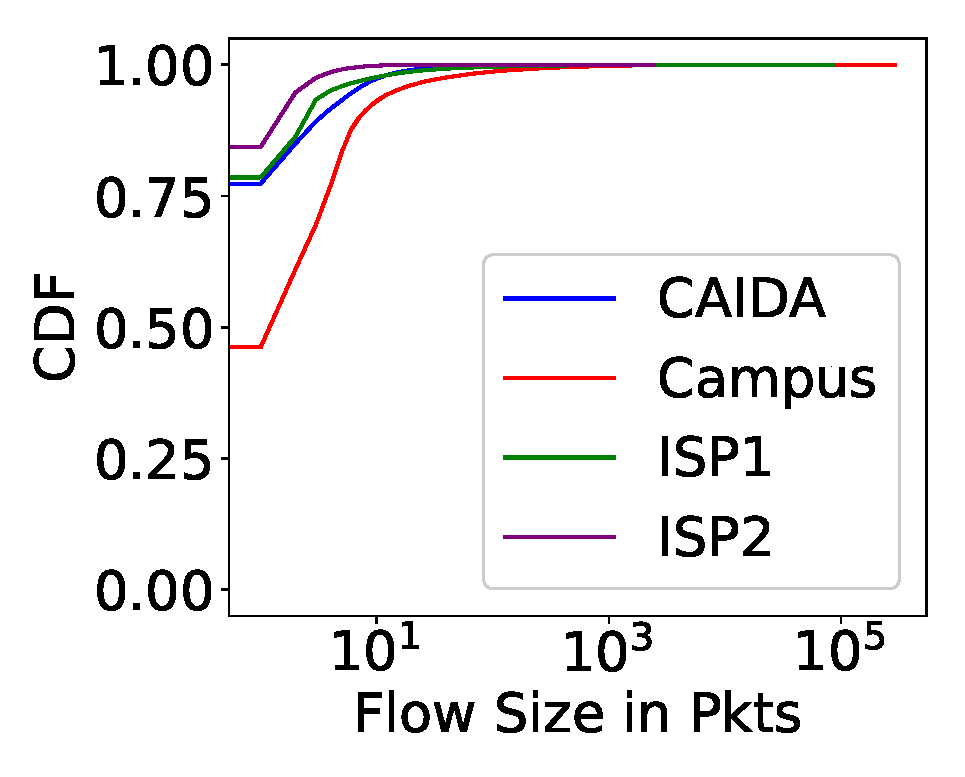
\includegraphics[width=\linewidth]{figures/exp84478/flow_size_distribution}
    \caption{Flow size distribution of the traces used for evaluation}
    \label{fig:flowsizedistribution}
\end{minipage}
\begin{minipage}{.45\linewidth}
	\centering
	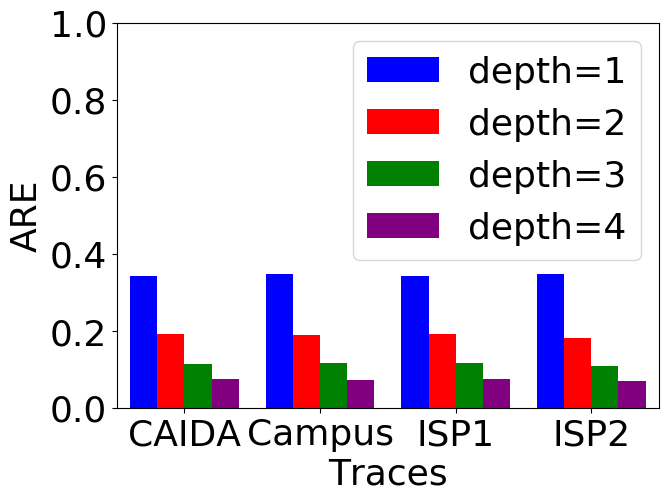
\includegraphics[width=\linewidth]{figures/exp84479/are_with_depth}
	\caption{Flow size estimation under different pipeline depth}
	\label{fig:comparison_increase_depth}
\end{minipage}
\end{figure}

Suppose $n$ flows are processed by each algorithm, where a flow is defined by the typical 5 tuples, i.e., source/destination IP addresses, protocol, and source/destination ports.
The measurement applications we use to evaluate the algorithms 
and traffic statistics we use as performance metrics are as follows. 

\begin{itemize}
    \item \emph{Flow Record Report.} 
An algorithm reports the flow records it maintains, 
where each record is of the form (flow ID, packet count). 
The performance metric we  use is \emph{Flow Set Coverage (FSC)} defined as 
\[FSC\!=\!\frac{\text{num. of flow records with complete flow IDs}}{n}.\]

    \item \emph{Flow Size Estimation.} 
Given a flow ID, an algorithm estimates the number of 
packets belonging to this flow. If no result can be reported, we use 0 as the default value. 
The performance metric we  use is \emph{Average Relative Error (ARE)} defined as 
\[ARE=\frac{1}{n}\sum\left|\frac{\text{estimated size of flow } i }{\text{real size of flow } i}-1\right|.\]

    \item \emph{Heavy Hitter Detection.} 
An algorithm reports heavy hitters, which are flows with more than $T$ packets, 
and $T$ is an adjustable parameter. 
Let $c_1$ be the number of  heavy hitters reported by an algorithm, 
$c_2$ the number of real heavy hitters, 
and among the reported $c_1$ heavy hitters $c$ of them are real.
The performance metric we use is \emph{F1 Score} defined as
\[\text{F1 Score}=\frac{2\cdot PR\cdot RR}{PR + RR},\]
where $PR = \frac{c}{c_1}$  and $RR=\frac{c}{c_2}$. 
We also use \emph{ARE} of the size estimation of the heavy hitters 
as another metric.

    \item \emph{Cardinality Estimation.} 
An algorithm estimates the number of flows. 
The performance metric we  use is \emph{Relative Error (RE)} defined as 
\[RE =\left|\frac{\text{estimated number of flows}}{n}-1\right|.\]
Notice that, linear counting\cite{whang_linear-time_1990} is used by ElasticSketch and HashFlow to estimate the number of flows in the count-min sketch and ancillary table respectively.


\end{itemize}

Following recommendations in the corresponding papers, we set the parameters of these algorithms as follows. 
\begin{itemize}
    \item HashPipe: We use 4 sub-tables of equal size.
    \item ElasticSketch: We adopt the hardware version, where 3 sub-tables
are used in its heavy part. The light part uses a count-min sketch of one array, 
and the two parts use the same number of cells.
    \item FlowRadar:  We use 4 hash functions for its bloom filter and 3 hash functions for its counting table.
The number of cells in the bloom filter is $40\times$ of that in the counting table. 
    \item HashFlow: We use the same number of cells in the main table and the ancillary table. 
The main table consists of three small hash tables with the weight $\alpha$ of 0.7. 
Each digest and counter in the ancillary table costs 8 bits.
\end{itemize}

We let these algorithms use the same amount of memory in all the experiments. 
For each flow record, we use a flow ID of 104 bits and a counter of 32 bits,
So 1 MB memory approximately corresponds to 60K flow records.
In the worst case, HashFlow, HashPipe and ElasticSketch (hardware version) will compute 4 hash results 
to access the corresponding cells, while FlowRadar always needs to compute 7 hash results. To save space, we use the acronyms presented in Table~\ref{table:acronyms} to denote the algorithms in figures when necessary. 

\begin{table}[ht!]
	\centering
	\caption{Acronyms for Algorithms}
	\label{table:acronyms}
	\begin{tabular} { c | c | c | c}
	\hline\hline
	Acronym & Algorithm & Acronym & Algorithm\\
	\hline
	HF & HashFlow & HP & HashPipe\\
%	\hline
%	HP & HashPipe\\
%	\hline
	ES & ElasticSketch & FR & FlowRadar\\
%	\hline
%	FR & FlowRadar\\
	\hline%\hline
	\end{tabular}
\end{table}


%Since we are interested in the flow sizes only, in the implementations we record the flow IDs (including source IP address, destination IP address, protocol, source port and destination port) and flow sizes (in packets) and omit other properties of flows. The data structure of HashFlow consists of 8 register arrays. While it is obvious that the width of five-tuple of flows is 104 bits, we allocate 32 bits to \emph{count} field in MT, 8 bits to \emph{digest} field and \emph{count} field in AT.





\subsection{Optimizing the Main Table and Ancillary Table }
We first demonstrate the performance of the main table with the collision resolution strategy, 
under different settings and parameters, i.e, using a multi-hash table, 
or using pipelined tables with different weights.

In Fig. \ref{fig:performance_comparison_hierarchical_hashtable}, there are 3 pipelined tables of which the weight is 0.6, 0.7 and 0.8 respectively and a multi-hash table. 
The traces are from  the campus network, and we increase the number of flows from 10K to 60K.
It can be seen that the pipelined tables with a weight around $\alpha=0.7$ achieves the best result.
Compared with the multi-hash table, it improves the \emph{FSC} by 3.1\%, 
and reduces the \emph{ARE} by 37.3\% respectively. 
This confirms our theoretical analysis on $\alpha$ in Section \ref{analysis}.
In the experiments thereafter, we will use a default weight of 0.7.


In Fig. \ref{fig:comparison_increase_depth}, we set the number of flow to 50K, and the depth of the main table is set to 1, 2, 3 and 4.
It can be seen that increasing $d$ from 1 to 3 reduces the \emph{ARE} by around 3 times (i.e., from 0.34 to 0.12), 
while increasing $d$ from 3 to 4 will have only a minor improvement (i.e., from 0.12 to 0.075). 
In the experiments thereafter, we will use a default depth of 3.


%As shown in Fig.~\ref{fig:comparison_increase_depth}, as the depth of MT increases from 1 to 4, the ARE (Average Relative Error) of \emph{flow size estimation} decreases from around 0.34 to around 0.075. However, we find that most of the improvement regarding the performance is achieved when the depth increases from 1 to 3 since the ARE is around 0.12 when the depth of MT is 3. Meanwhile, by increasing the depth from 3 to 4, we will have to take the risk of doing one more hash computation and one more memory read operation. so we believe that it is a good tradeoff to constrain the time complexity and give up the benefits of more depths. We will set the default depth of MT to 3. 

\begin{figure}[ht!]
    \centering
    \mbox{
        \subfigure[Flow Record Report\label{MT-flowrecord}]{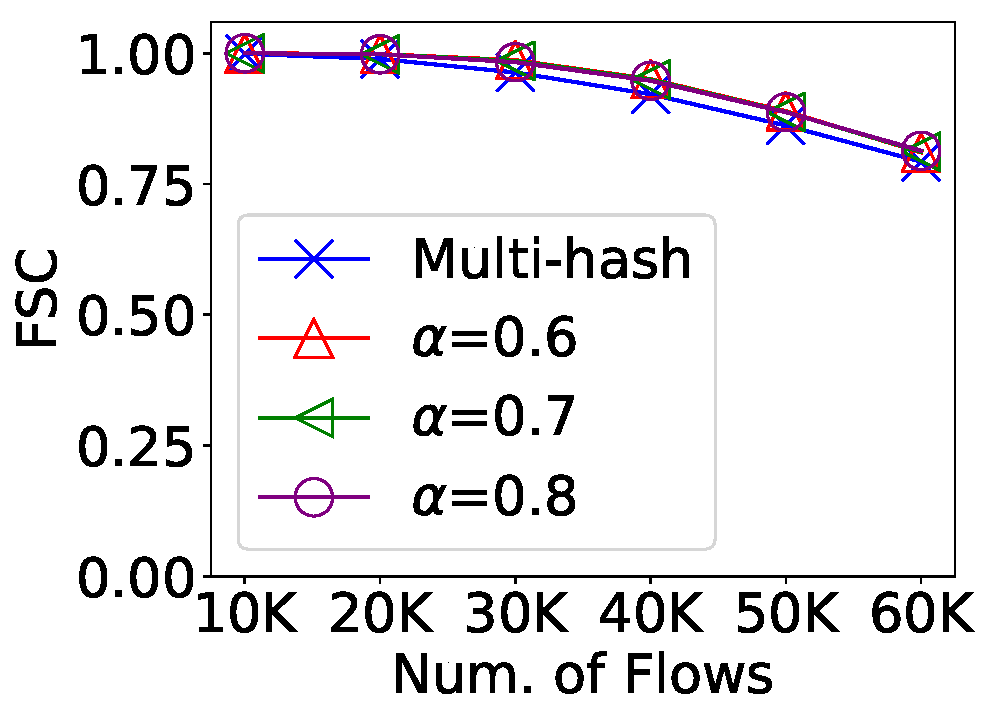
\includegraphics[width=0.45\linewidth]{figures/exp84454/flow_monitoring_fsc}}
        \subfigure[Flow Size Estimation\label{MT-flowsize}]{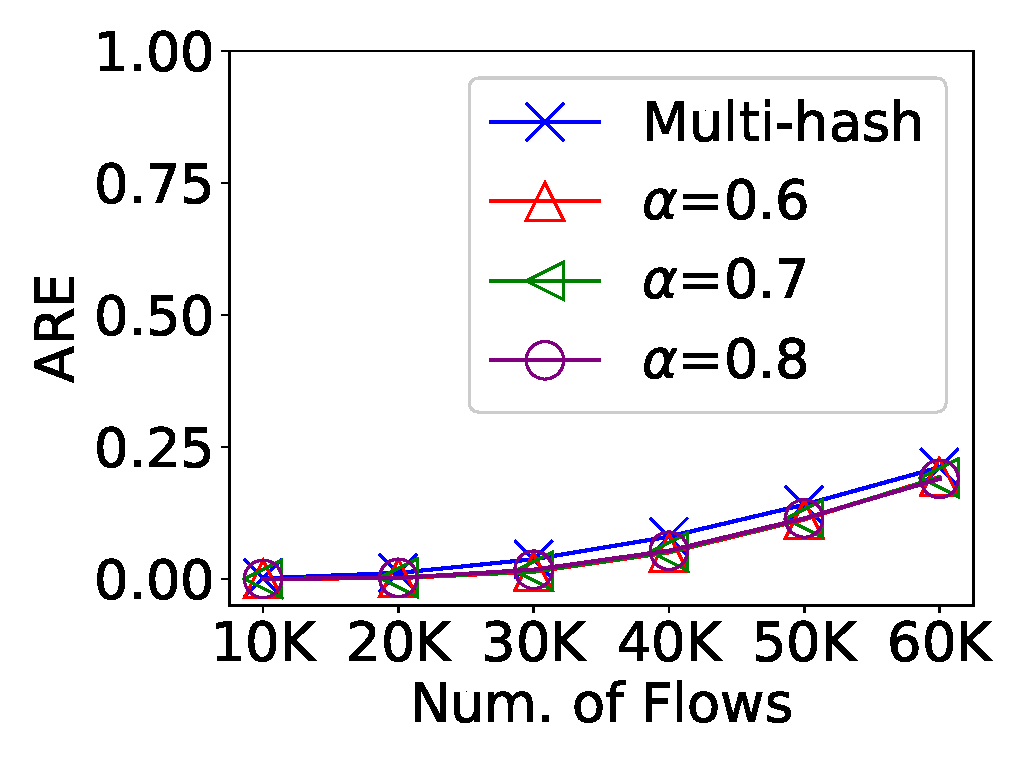
\includegraphics[width=0.45\linewidth]{figures/exp84454/flow_size_estimation_are}}
    }
    \caption{Comparing multi-hash table with pipelined tables.}
    \label{fig:performance_comparison_hierarchical_hashtable}
\end{figure}

To evaluate the influence that the size of ancillary table has upon HashFlow, we define a parameter $\beta$ and let $n_2=n_1\times\beta$, where $n_1$ and $n_2$ are number of buckets in the main table and ancillary table respectively. There is not an ancillary table at all when $\beta=0.0$. We feed a number of flows extracted from CAIDA file, and calculate the F1 Score and ARE (Average Relative Error) of heavy hitter detection where a heavy hitter is a flow with no less than 10 packets. Fig.~\ref{fig:are_for_various_beta} shows that the ancillary table is crucial for the performance of HashFlow and normally $\beta=0.5$ is good enough. However, when attacks such as DDoS occur, the accumulation of elephant flows in ancillary table will be interrupted frequently. To be robust when facing such attacks, in the following experiments we  set $\beta$ to 1.0 by default.

\begin{figure}[ht!]
	\centering
	\mbox{
		\subfigure[F1 Score\label{hhd_f1_score}]{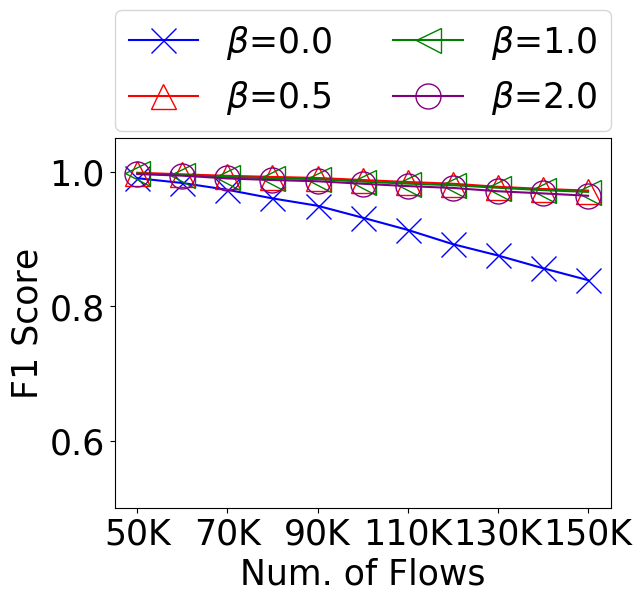
\includegraphics[width=0.45\linewidth]{figures/exp84493/caida_heavy_hitter_detection_f1_score}}
		\subfigure[ARE\label{hhd_ARE}]{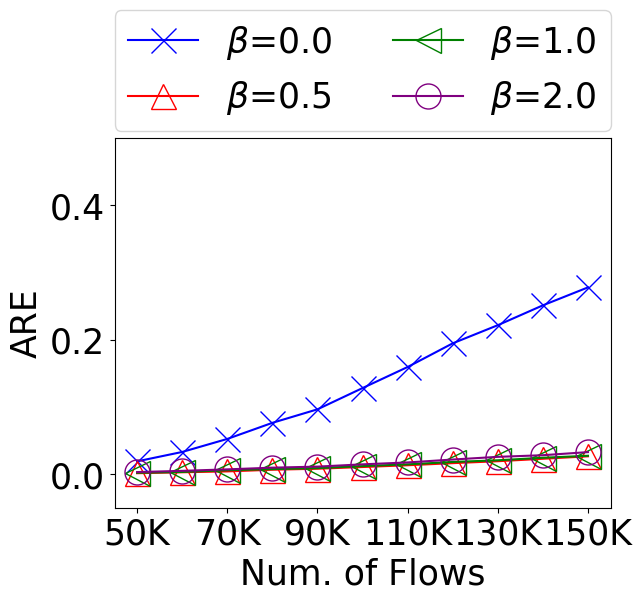
\includegraphics[width=0.45\linewidth]{figures/exp84493/caida_heavy_hitter_detection_are}}
	}
	\caption{F1 Score and Average Relative Error (ARE) of heavy hitter detection when the size of ancillary table varies.}
	\label{fig:are_for_various_beta}
\end{figure}




\subsection{Application Performance }
In this section, we evaluate the performance of HashFlow against HashPipe, ElasticSketch and FlowRadar, 
for typical measurement applications as described in  Section~\ref{methodology}.

Fig.~\ref{fig:comparison_concurrent_flows_increases_flow_monitoring} shows that HashFlow nearly always performs better than the others in the sense of \emph{Flow Set Coverage (FSC)}. For example, 
for a total of 250K flows, it can successfully report around 55K flows, 
nearly making a full use of its main table. 
Its \emph{FSC} is more than 20\% higher than ElasticSketch in all traces, 
and is that higher than HashPipe in the Campus Network trace. 
The only exception when HashFlow loses is that, 
for a very small number of flows (the left up corner in the figures), 
FlowRadar has the highest coverage. 
This is because FlowRadar can successfully decode nearly all flow records when only a few flows arrive. 
But its performance drops significantly soon after the flow count goes beyond a certain point, 
since after that, too many flows mixed up, and the decoding often fails.

\begin{figure*}[ht!]
    \centering
    \mbox{
    \subfigure[CAIDA\label{subfig:caidaflowmonitoring}]{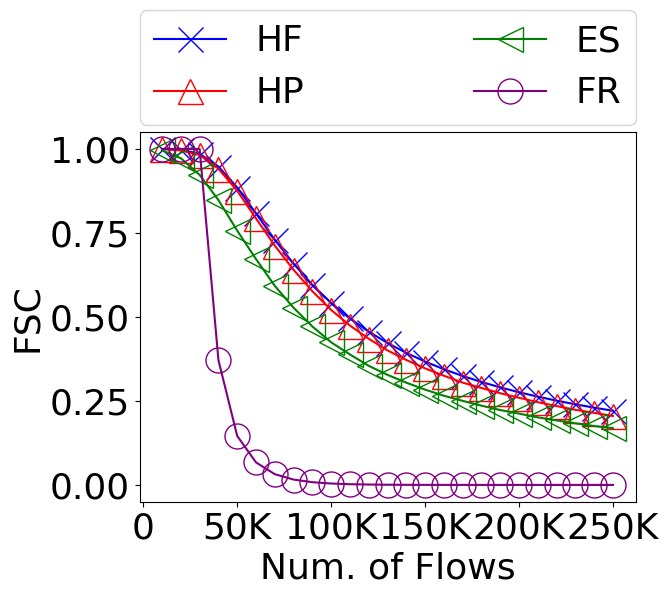
\includegraphics[width=0.24\linewidth]{figures/exp84485/caida_flow_monitoring_fsc}}
    \subfigure[Campus Network\label{subfig:campusnetworkflowmonitoring}]{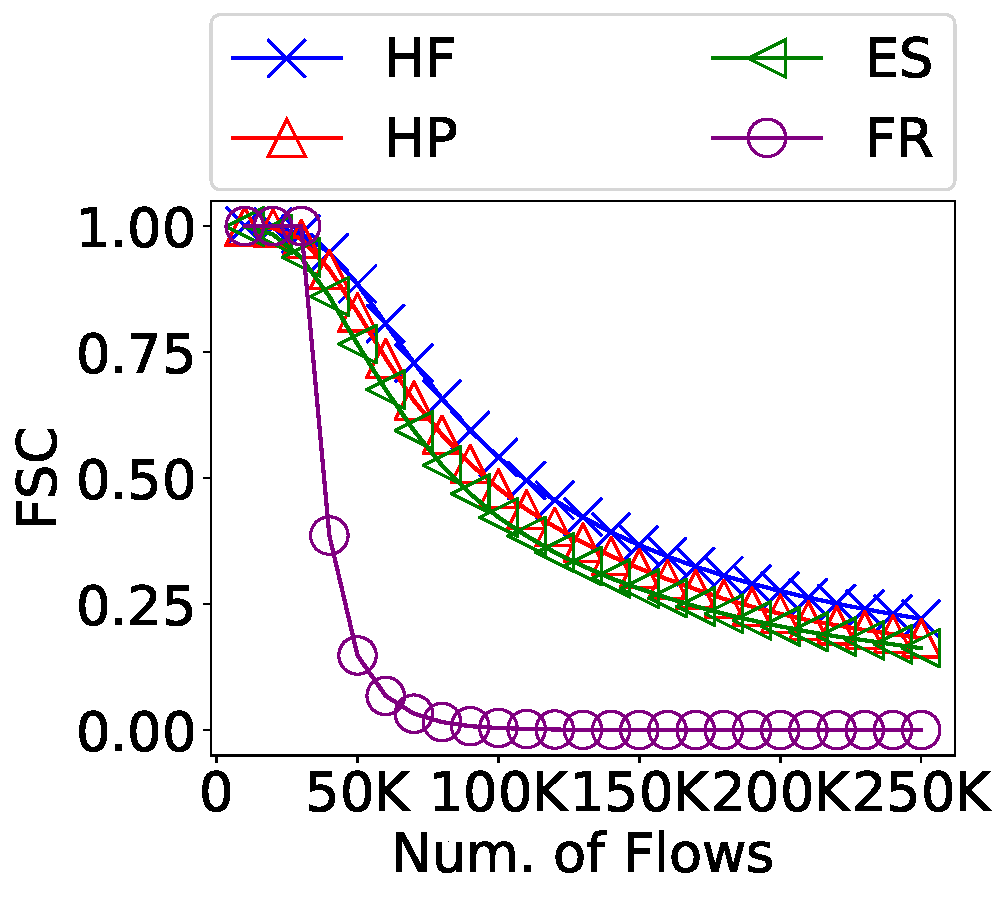
\includegraphics[width=0.24\linewidth]{figures/exp84485/tsinghua_flow_monitoring_fsc}}
    \subfigure[ISP1\label{subfig:hgcflowmonitoring}]{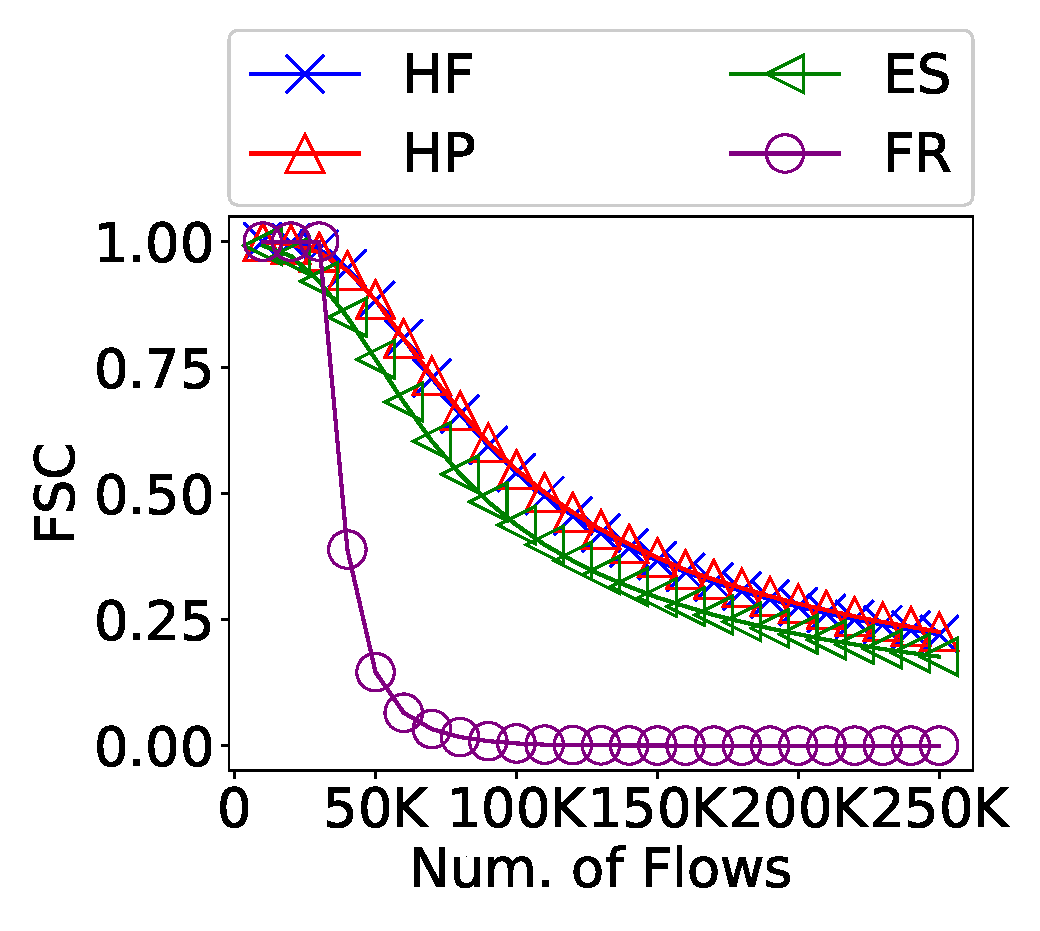
\includegraphics[width=0.24\linewidth]{figures/exp84485/hgc_flow_monitoring_fsc}}
    \subfigure[ISP2\label{subfig:telecomflowmonitoring}]{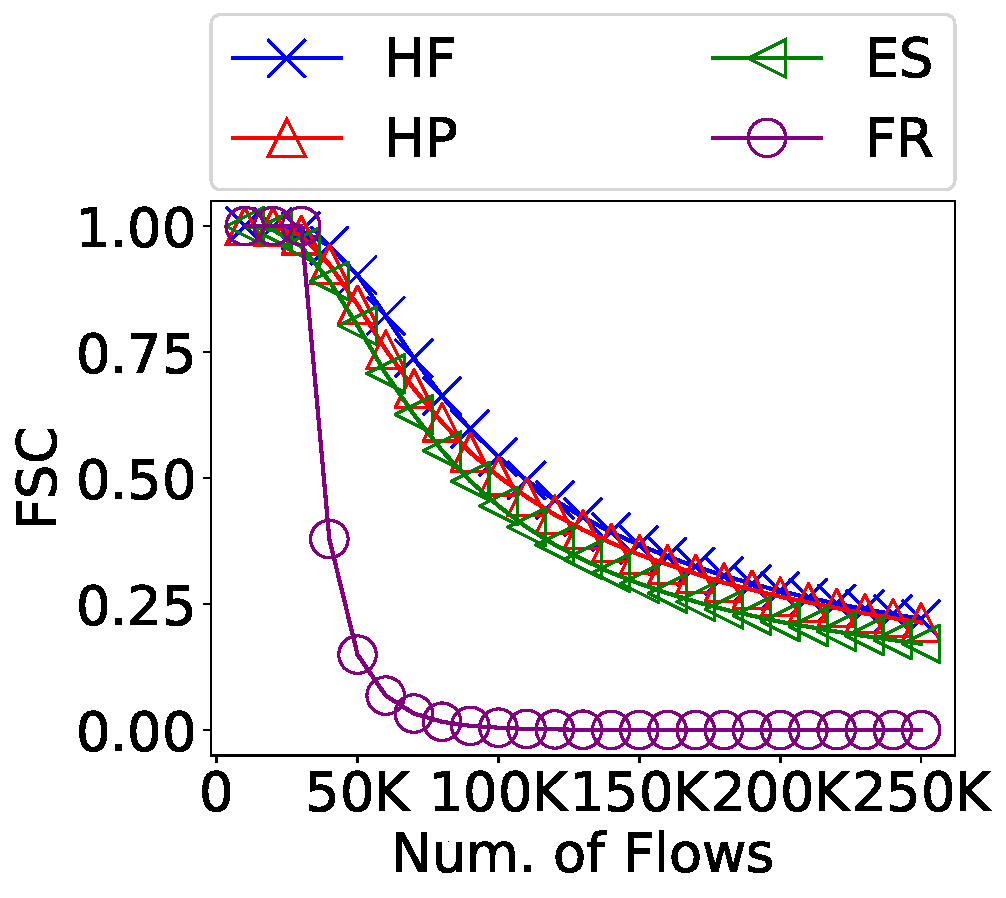
\includegraphics[width=0.24\linewidth]{figures/exp84485/telecom_flow_monitoring_fsc}}
    }
    \caption{\emph{Flow Set Coverage (FSC)} for \emph{Flow Record Report}}
    \label{fig:comparison_concurrent_flows_increases_flow_monitoring}
\end{figure*}

Fig.~\ref{fig:comparison_concurrent_flows_increases_cardinality} shows the results 
of estimating the total number of flows, where in most of the time, 
HashFlow, ElasticSketch and FlowRadar achieve a similar level of accuracy. 
Among them, FlowRadar works slightly better since it uses a bloom filter to count flows, 
which is not sensitive to flow sizes, while HashFlow and ElasticSketch are slightly affected 
by the flow size distribution due to their assumption on the existence of elephant and mice flows. 
This is particularly true in the ISP2 trace, where nearly all flows contain less than 5 packets.
HashPipe always performs badly since it does not use any advanced cardinality estimation technique 
to compensate for the flows it drops. 

\begin{figure*}[ht!]
    \centering
    \mbox{
        \subfigure[CAIDA\label{subfig:caidacardinality}]{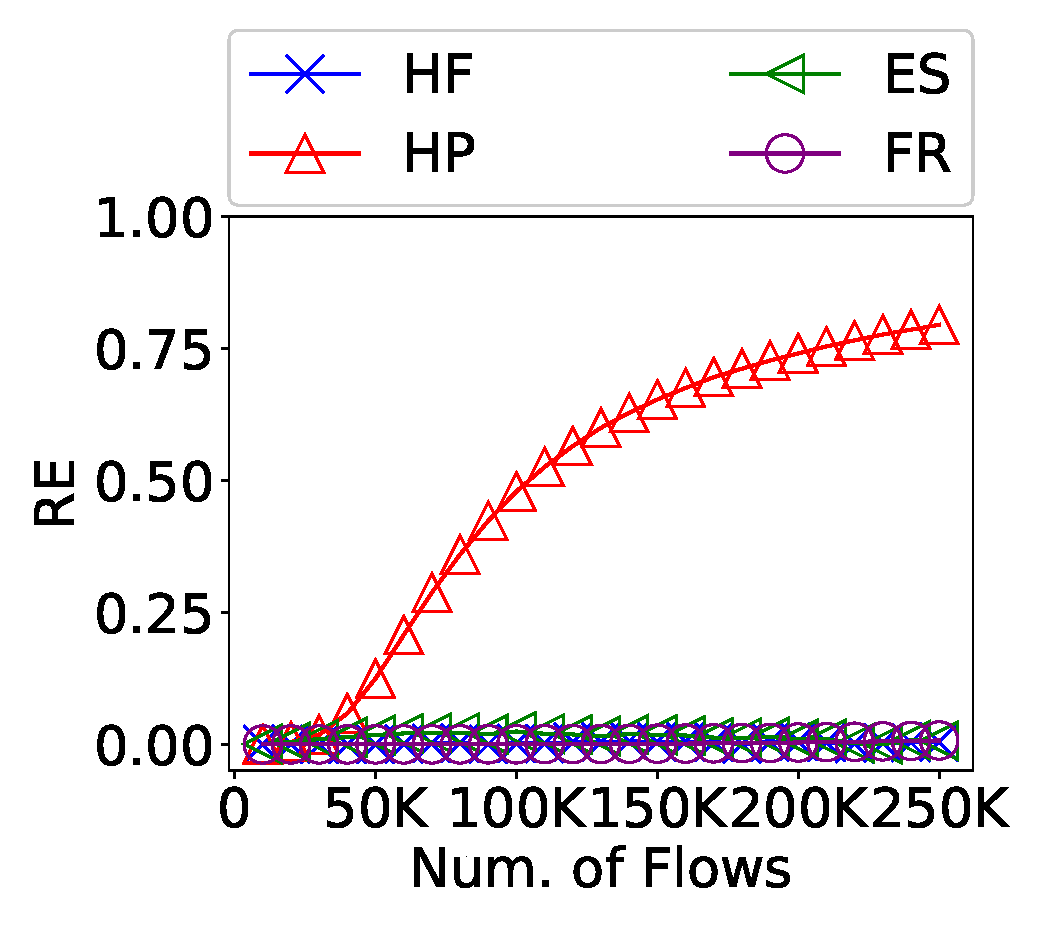
\includegraphics[width=0.24\linewidth]{figures/exp84485/caida_cardinality_re}}
        \subfigure[Campus Network\label{subfig:campusnetworkcardinality}]{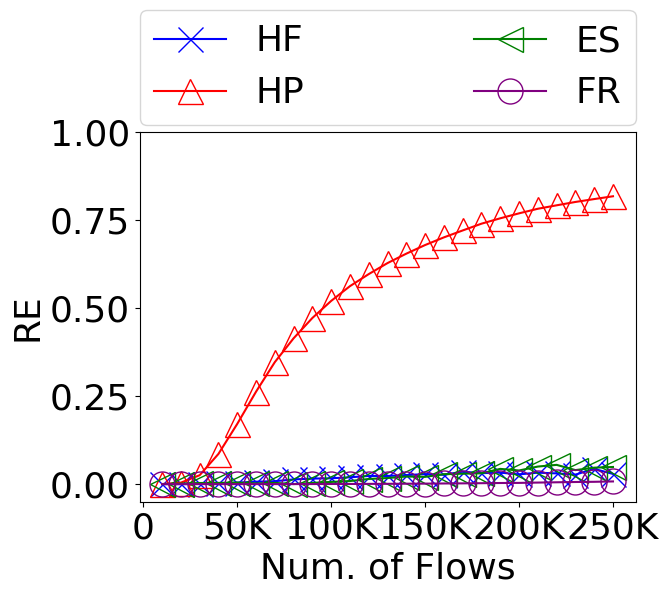
\includegraphics[width=0.24\linewidth]{figures/exp84485/tsinghua_cardinality_re}}
        \subfigure[ISP1\label{subfig:hgccardinality}]{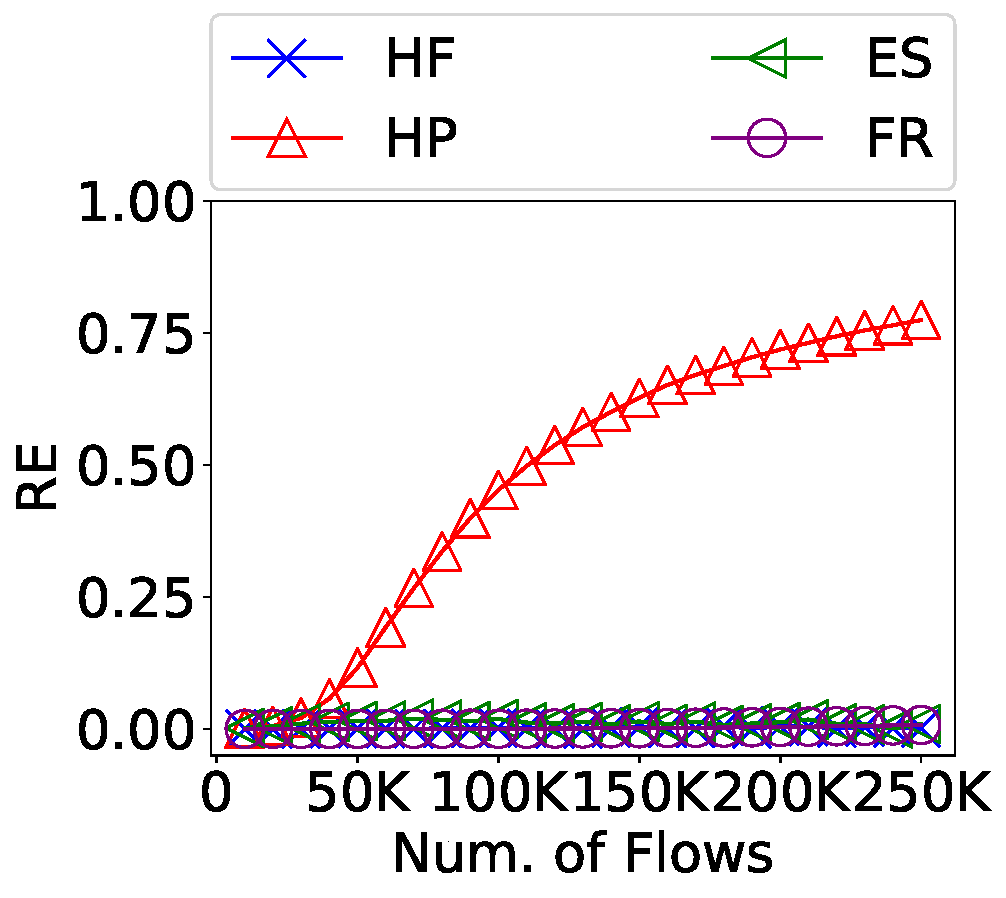
\includegraphics[width=0.24\linewidth]{figures/exp84485/hgc_cardinality_re}}
        \subfigure[ISP2 Trace\label{subfig:telecomcardinality}]{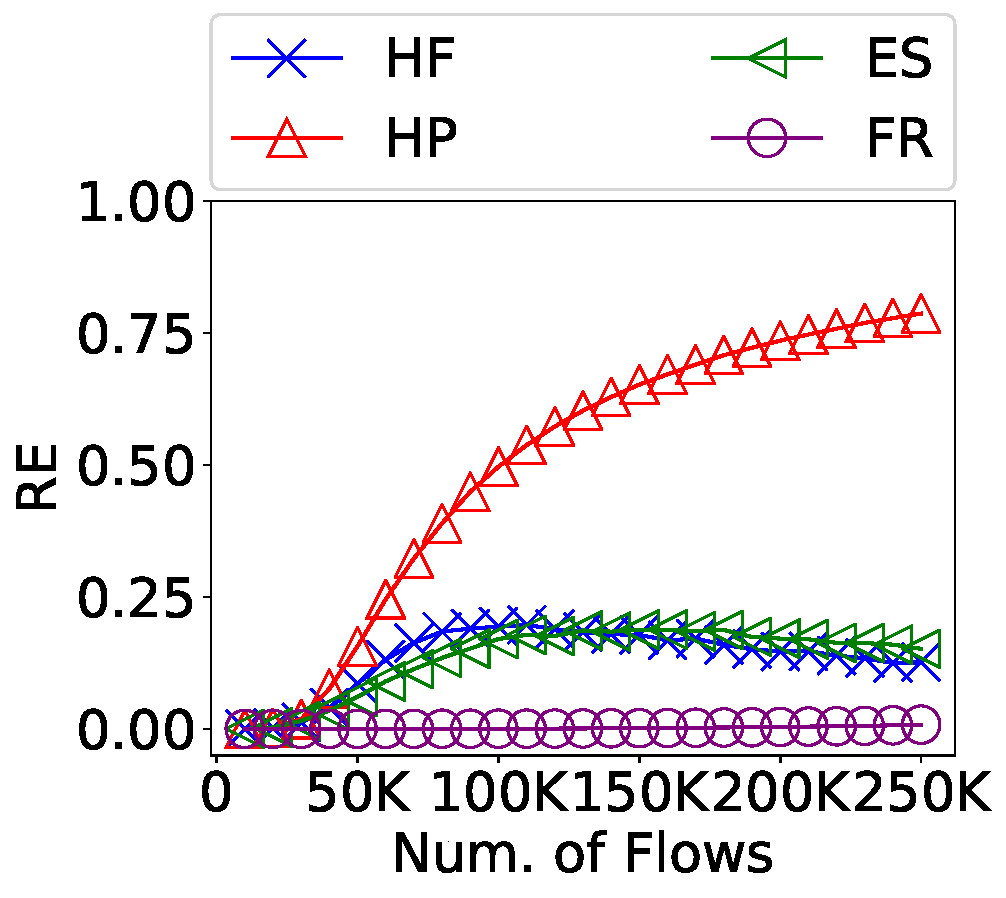
\includegraphics[width=0.24\linewidth]{figures/exp84485/telecom_cardinality_re}}
    }
    \caption{\emph{Relative Error (RE)} for \emph{Flow Cardinality Estimation}}
    \label{fig:comparison_concurrent_flows_increases_cardinality}
\end{figure*}

Fig. \ref{fig:comparison_concurrent_flows_increases_fs_estimation} 
shows that HashFlow often achieves a much lower estimation error 
than its competitors when estimating the flow sizes. For example, when there are 100K flows, the relative estimation error
of HashFlow is around 0.4, while the error of the others is more than 0.6 (50\% higher) in most cases. 
FlowRadar performs very badly when there are more than 40K flows, 
while the accuracy of HashPipe is not very stable.


\begin{figure*}[ht!]
    \centering
    \mbox{
        \subfigure[CAIDA Trace\label{subfig:caidafsestimation}]{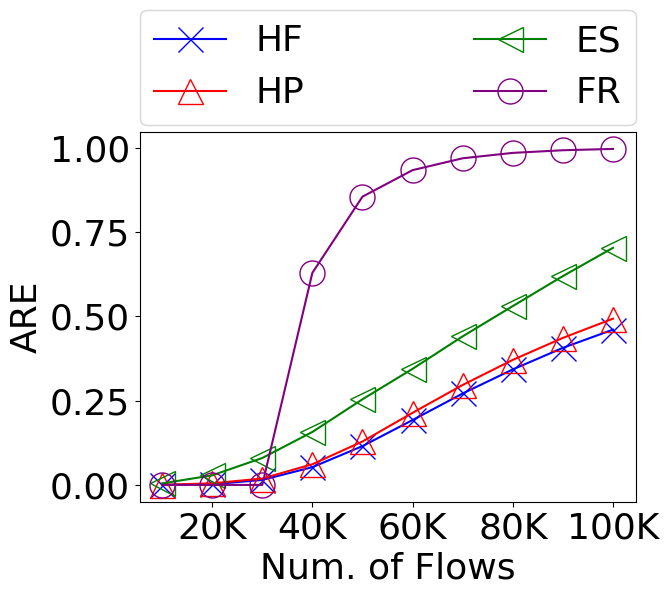
\includegraphics[width=0.24\linewidth]{figures/exp84485/caida_flow_size_estimation_are}}
        \subfigure[Campus Network Trace\label{subfig:campusnetworkfsestimation}]{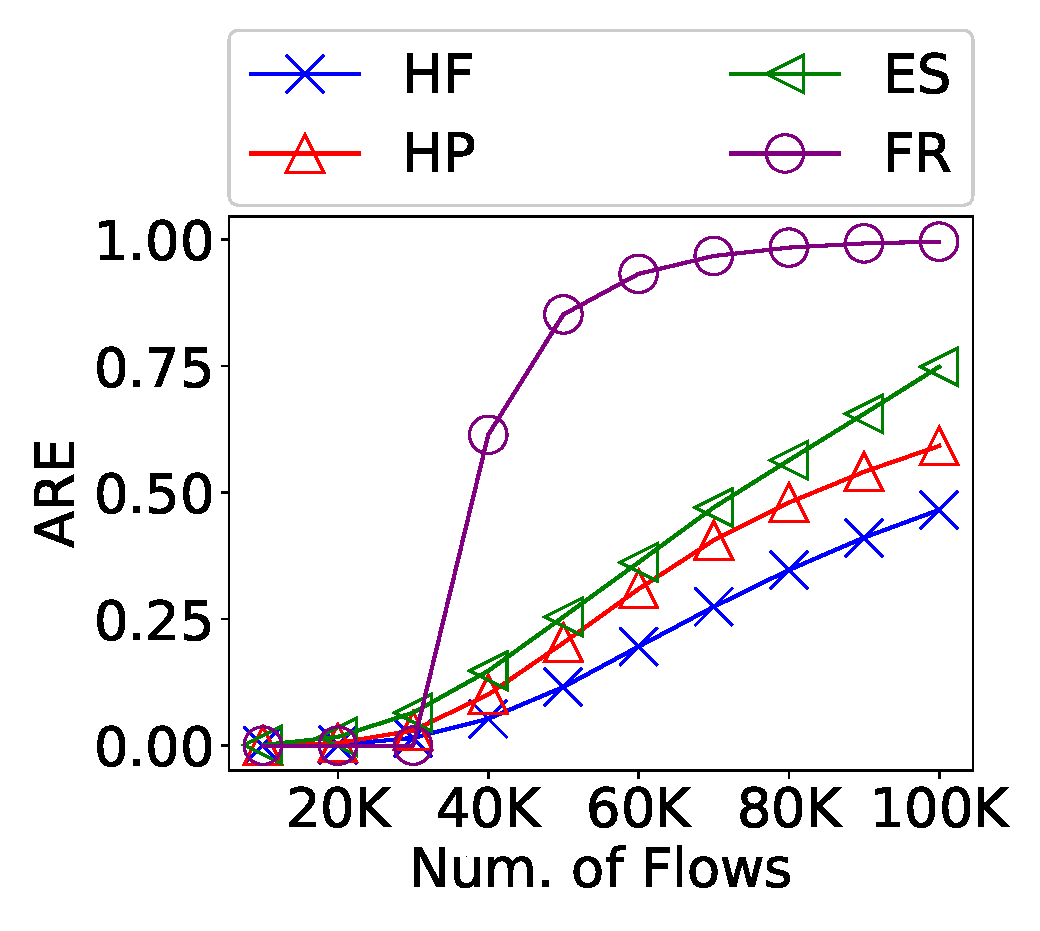
\includegraphics[width=0.24\linewidth]{figures/exp84485/tsinghua_flow_size_estimation_are}}
        \subfigure[HGC Trace\label{subfig:hgcfsestimation}]{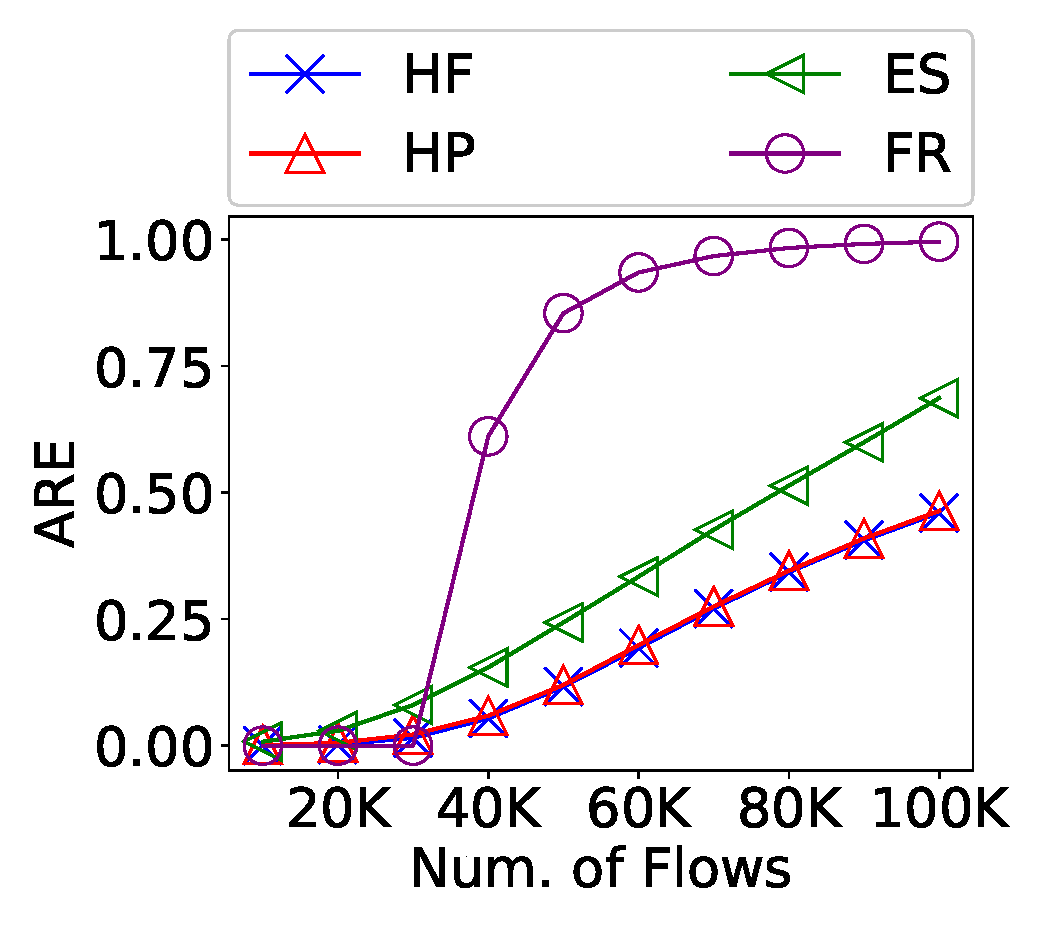
\includegraphics[width=0.24\linewidth]{figures/exp84485/hgc_flow_size_estimation_are}}
        \subfigure[Telecom Trace\label{subfig:telecomfsestimation}]{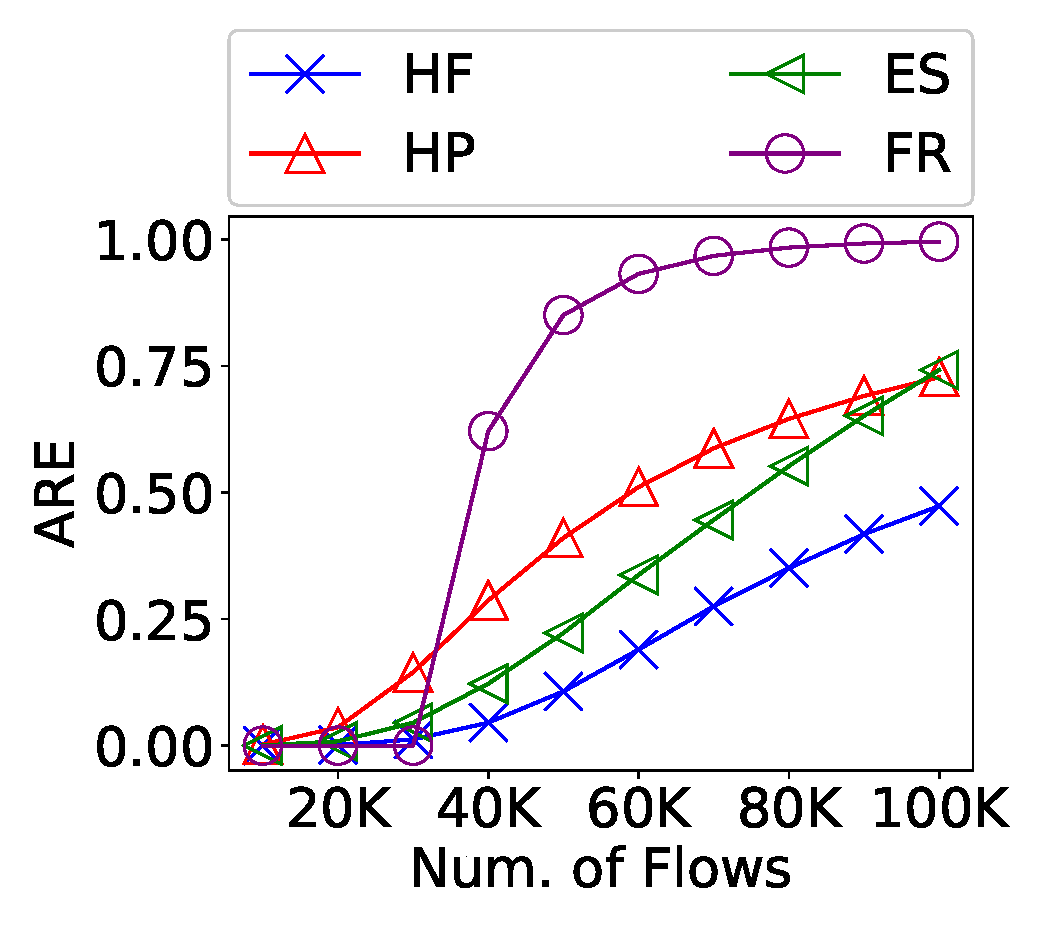
\includegraphics[width=0.24\linewidth]{figures/exp84485/telecom_flow_size_estimation_are}}
    }
    \caption{\emph{Average Relative Error (ARE)} for \emph{Flow Size Estimation}}
    \label{fig:comparison_concurrent_flows_increases_fs_estimation}
\end{figure*}

At last, we show whether they can accurately detect heavy hitters.
We feed 250K flows to each algorithm, and calculate the \emph{F1 Score} of their detection accuracy as well as the $ARE$ of the estimated sizes of the detected heavy hitters.
%where the threshold for a flow to be treated as a heavy hitter varies. 
The results are depicted in Fig. \ref{fig:comparison_concurrent_flows_increases_hhd_f1_score} 
and Fig.~\ref{fig:comparison_concurrent_flows_increases_hhd_are}, respectively. 
Apparently, FlowRadar is not a good candidate under such heavy load. 
HashPipe is designed specifically for detecting heavy hitters, 
but our HashFlow still outperforms it in nearly all cases, for both metrics. 
Not considering the extreme case of the ISP2 trace where most flows are typically very small, 
for a wide range of thresholds, HashFlow achieves a \emph{F1 Score} of 1 (accurately detecting all heavy hitters) 
when the scores of HashPipe and ElasticSketch are around 0.9 and 0.4 $\sim$ 0.7, respectively. 
On the other hand, when HashFlow makes nearly perfect size estimation of the heavy hitters, 
the \emph{ARE} of HashPipe and ElasticSketch are around 0.15 $\sim$ 0.2 and 0.2 $\sim$ 0.25, respectively.
Even with a very small threshold used in the ISP2 trace, HashFlow clearly outperforms the others.

\begin{figure*}[ht!]
    \centering
    \mbox{
        \subfigure[CAIDA\label{subfig:caidahhdf1score}]{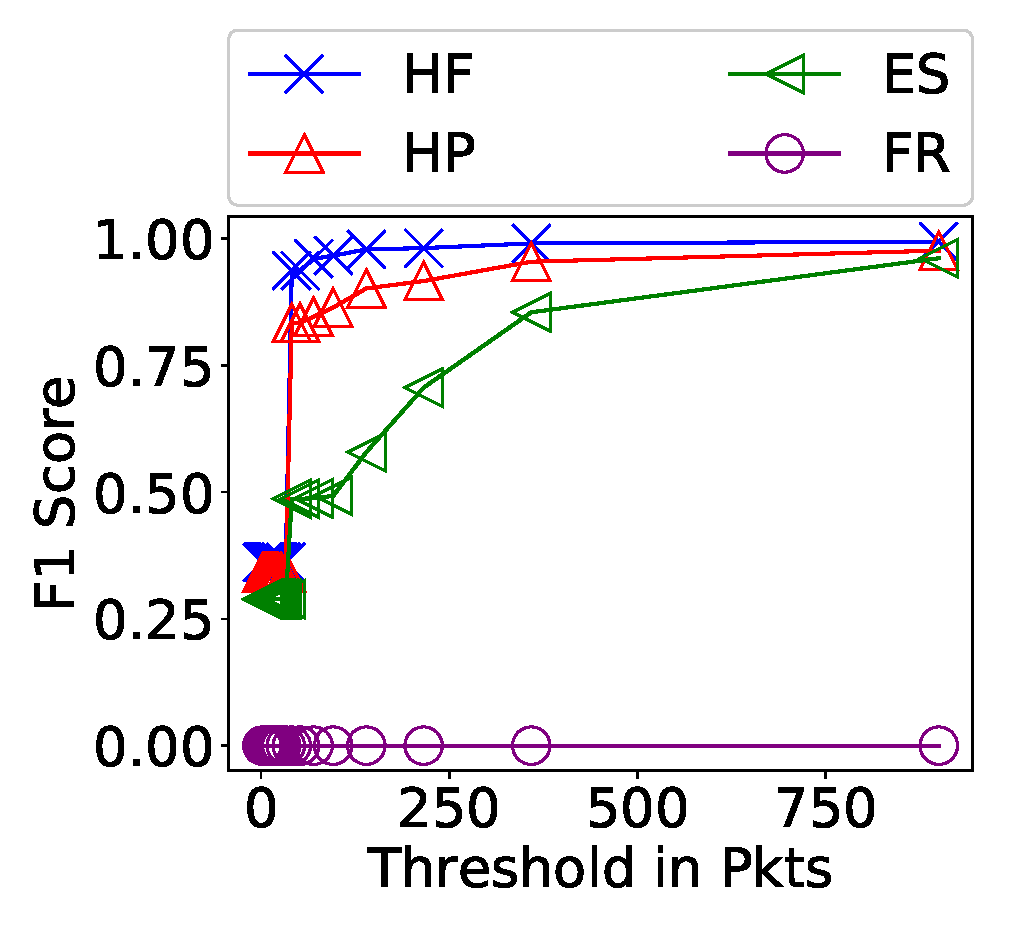
\includegraphics[width=0.24\linewidth]{figures/exp84486/caida_250K_f1_score}}
        \subfigure[Campus Network\label{subfig:campusnetworkhhdf1score}]{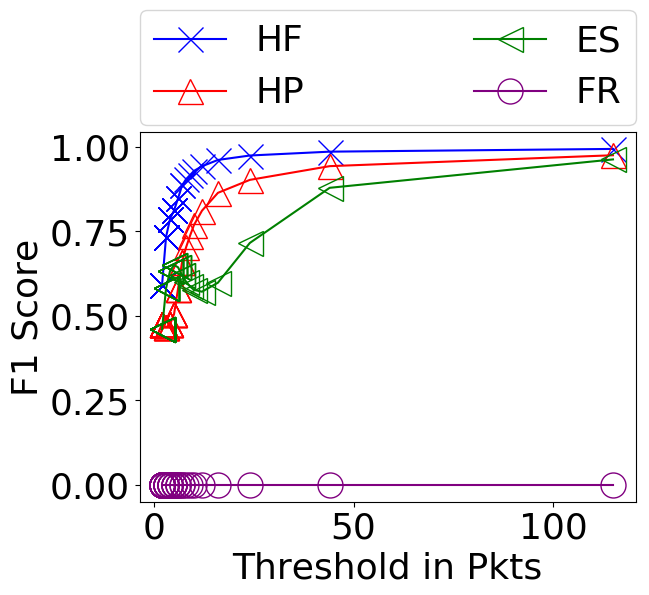
\includegraphics[width=0.24\linewidth]{figures/exp84486/tsinghua_250K_f1_score}}
        \subfigure[ISP1\label{subfig:hgchhdf1score}]{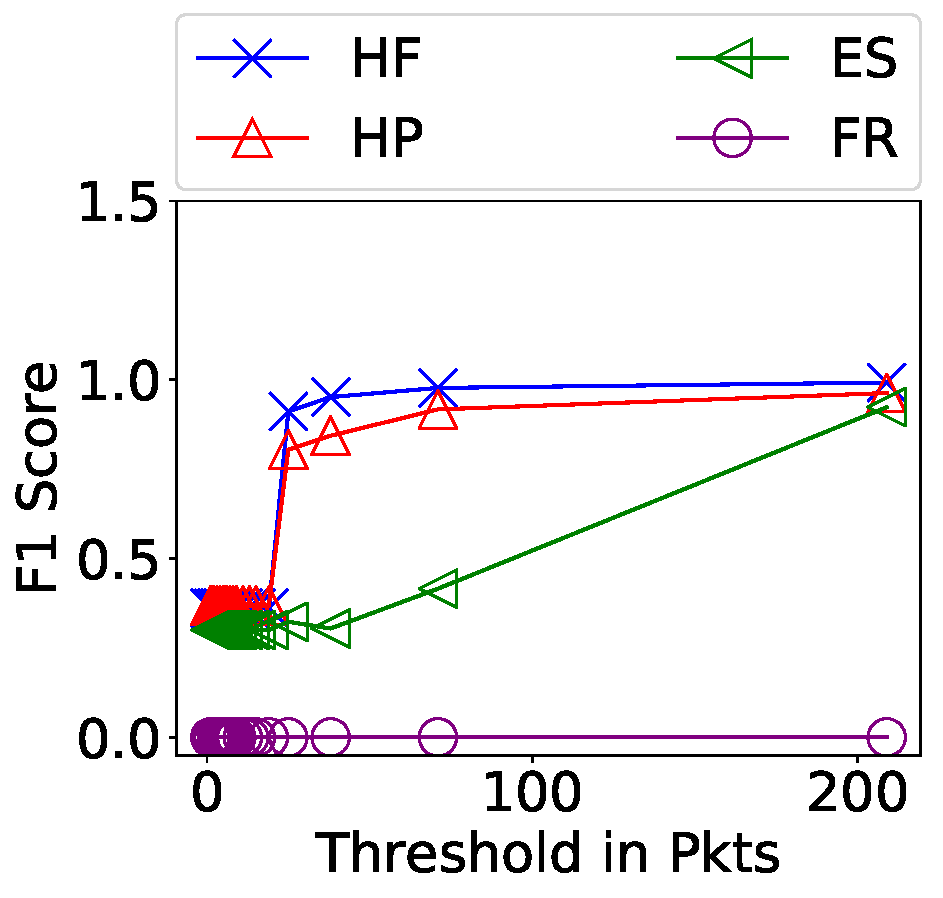
\includegraphics[width=0.24\linewidth]{figures/exp84486/hgc_250K_f1_score}}
        \subfigure[ISP2\label{subfig:telecomhhdf1score}]{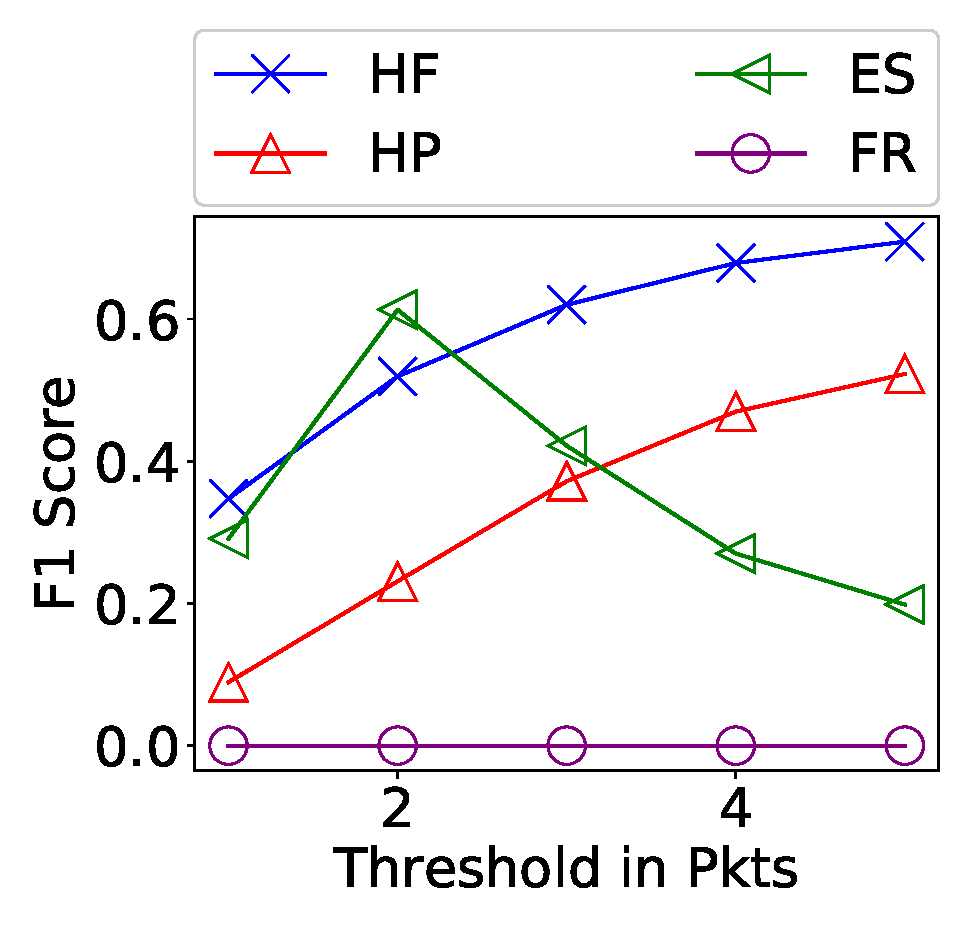
\includegraphics[width=0.24\linewidth]{figures/exp84486/telecom_250K_f1_score}}
    }
    \caption{\emph{F1 Score} for \emph{Heavy Hitter Detection}}
    \label{fig:comparison_concurrent_flows_increases_hhd_f1_score}
\end{figure*}


\begin{figure*}[ht!]
    \centering
    \mbox{
        \subfigure[CAIDA\label{subfig:caidahhdare}]{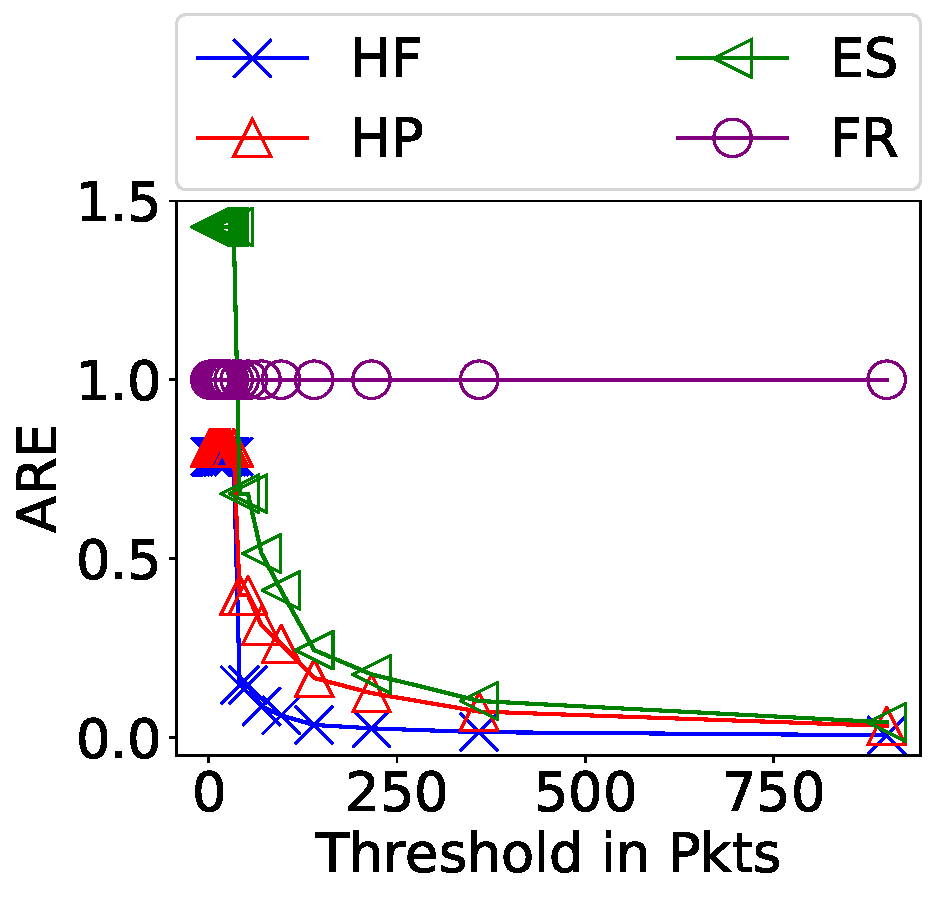
\includegraphics[width=0.24\linewidth]{figures/exp84486/caida_250K_re}}
        \subfigure[Campus Network\label{subfig:campusnetworkhhdare}]{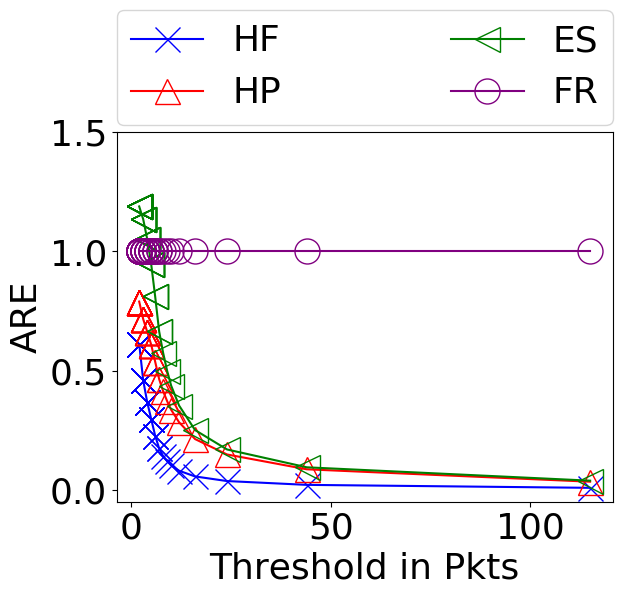
\includegraphics[width=0.24\linewidth]{figures/exp84486/tsinghua_250K_re}}
        \subfigure[ISP1\label{subfig:hgchhdare}]{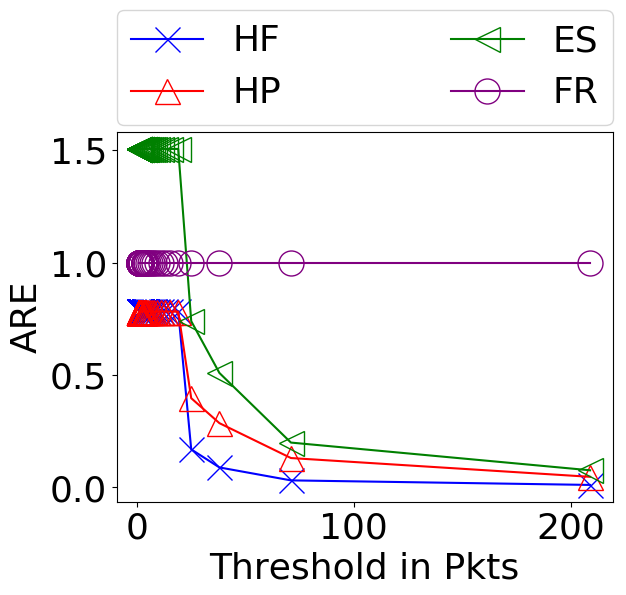
\includegraphics[width=0.24\linewidth]{figures/exp84486/hgc_250K_re}}
        \subfigure[ISP2\label{subfig:telecomhhdare}]{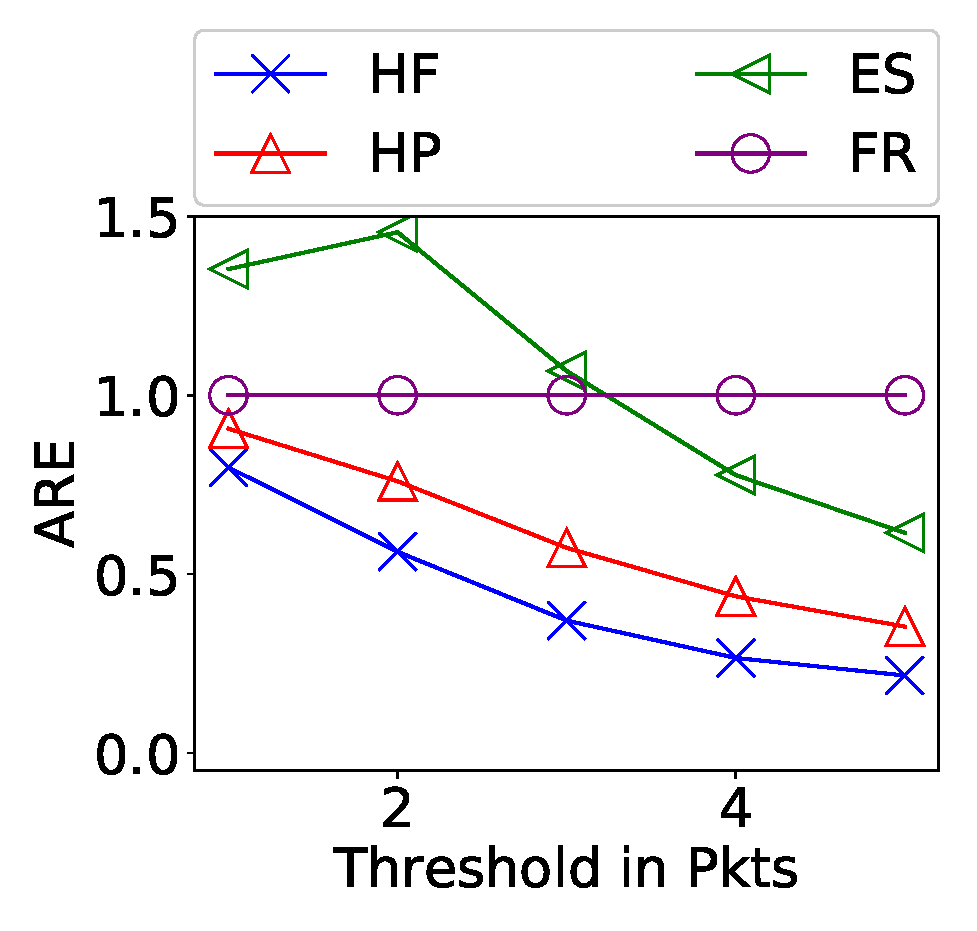
\includegraphics[width=0.24\linewidth]{figures/exp84486/telecom_250K_re}}
    }
    \caption{\emph{Average Relative Error(ARE)} for \emph{Heavy Hitter Detection}}
    \label{fig:comparison_concurrent_flows_increases_hhd_are}
\end{figure*}

\subsection{Throughput}
\label{subsec:throughput}
\begin{figure*}[ht!]
	\centering
	\mbox{
		\subfigure[Throughput\label{fig:throughput}]{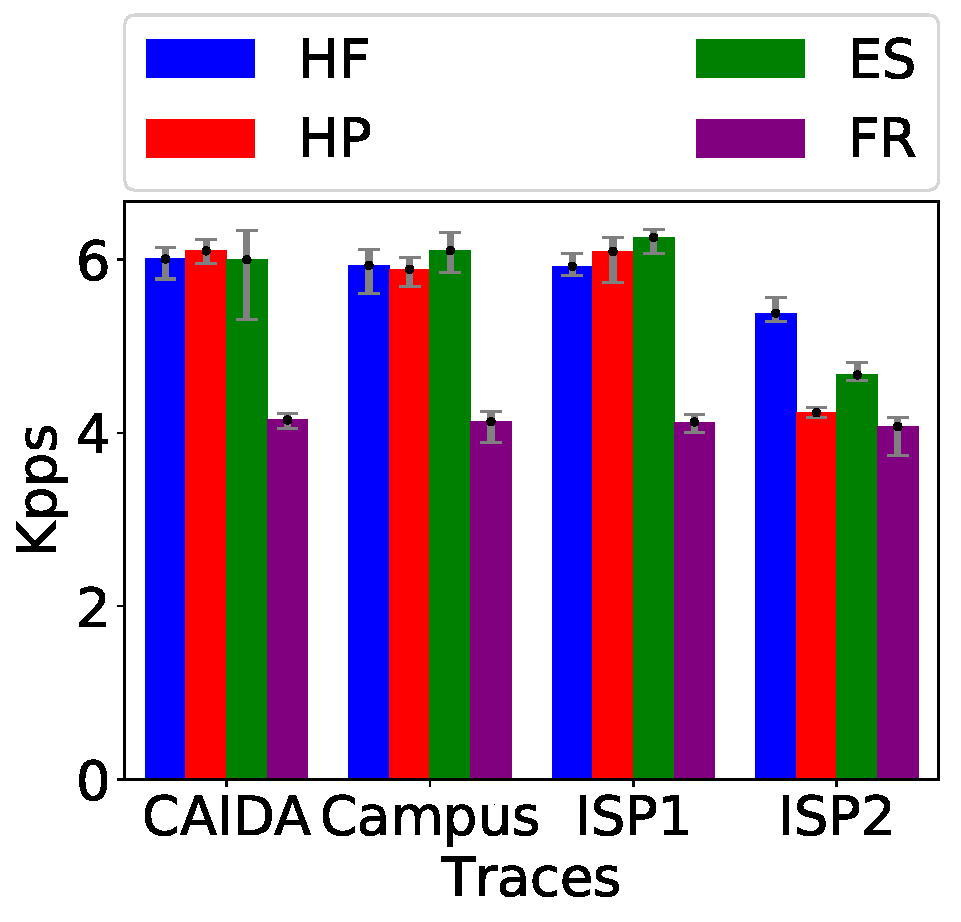
\includegraphics[width=0.24\linewidth]{figures/exp84484/throughput}}
		\subfigure[Number of hash operations\label{fig:avehash}]{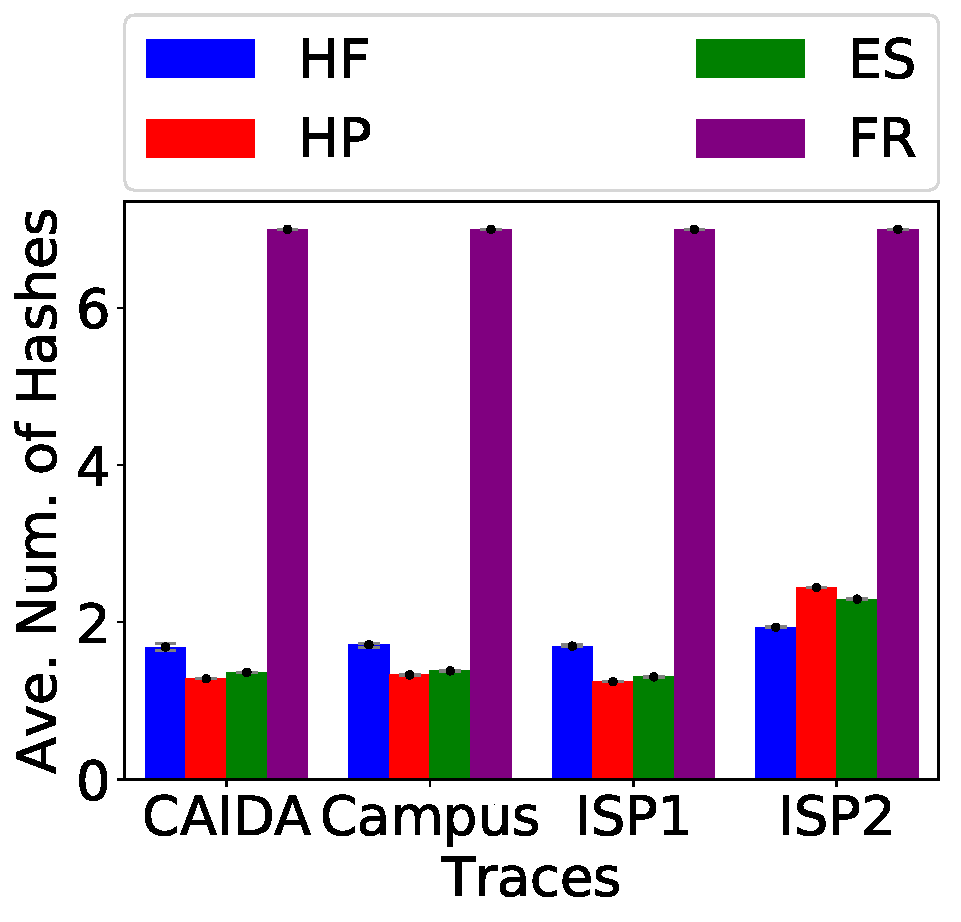
\includegraphics[width=0.24\linewidth]{figures/exp84490/ave_hash}}
		\subfigure[Number of memory accesses\label{fig:avemem}]{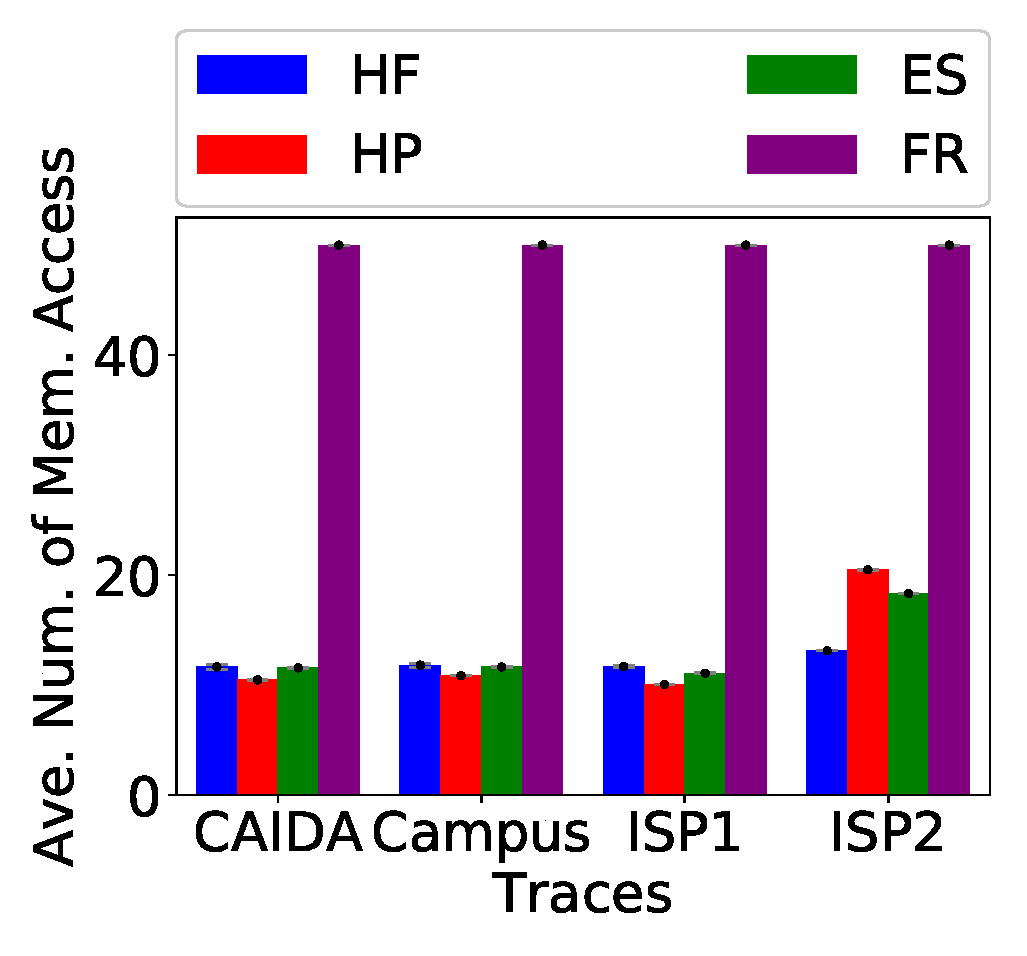
\includegraphics[width=0.24\linewidth]{figures/exp84490/ave_mem}}
		\subfigure[Resubmit Rate\label{fig:increaseinprocessing}]{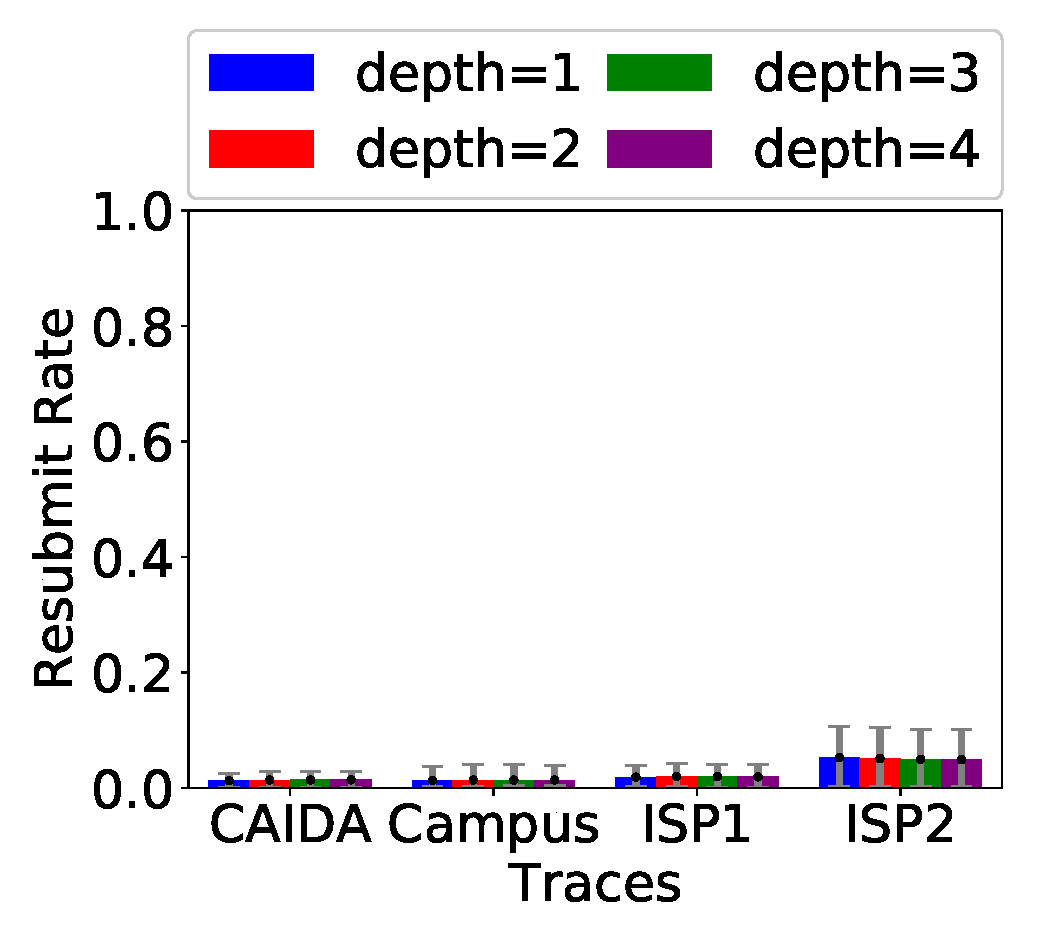
\includegraphics[width=0.24\linewidth]{figures/exp84491/increase_in_processing}}
	}
	\caption{Throughput, Hash Operation, Memory Access and Increase in Processing}
	\label{throughput}
\end{figure*}
We test the throughput of these algorithms with bmv2, 
on a PC with Intel(R) Core(TM) i5-4680K CPU@3.40GHz, 
where each CPU core owns a 6144 KB cache. 
We  use \emph{isolcpus} to isolate the cores to prevent context switches.
Bmv2 achieves around 20 Kpps forwarding speed, 
and the throughput after loading the algorithms are depicted in Fig. \ref{fig:throughput}.
To obtain a better understanding, we also record the average number of 
hash operations, as well as memory accesses, for each algorithm. 
The  results in Fig. \ref{fig:avehash} and Fig. \ref{fig:avemem} indicate that, 
HashFlow will perform comparably to HashPipe and ElasticSketch, 
and much better than FlowRadar, in the sense of the number of memory accesses and hash operations.

In our hardware implementation, the only risk degrading the throughput of the switch is that some packets will be resubmitted (or recirculated), so the switch will have to process more packets than those transmitted through it. To evaluate the possible loss of throughput, we calculate the \emph{Resubmit Rate} defined as 
%$\text{Resubmission Rate}=\frac{n_2}{n_1}.$
\begin{eqnarray*}
\text{Resubmit Rate}=\frac{n_2}{n_1}.
\end{eqnarray*}
where $n_1$ is the number of packets arriving at the switch, and $n_2$ is the number of packets that are resubmitted.

As shown in Fig.~\ref{fig:increaseinprocessing}, when there are 100K flows fed into the switch, the \emph{Resubmit Rate} is normally less than 2\%, and it is no more than 5.2\% in the trace provided by ISP2, which is far less skewed than the real network traffic. So HashFlow will achieve very good performance and the loss of throughput is negligible.


%calculate the average number of memory accesses and hash computations for processing a packet. As shown in Fig.~\ref{fig:avehash}, the average number of hash computations of HashFlow is slightly greater than the other 3 algorithms on the first 3 traces. For example, the average number of computations of HashFlow is 23.5\% and 31.2\% greater than that of ElasticSketch and HashPipe respectively on the CAIDA trace. That's because ElasticSketch and HashPipe allows a flow record to be cached in multiple positions of the data structure, so a elephant flow is more likely to be cached in the starting sub-tables, avoiding making more hash computations and traversing deep into the sub-tables, while a elephant stored the the last sub-table by HashFlow will always be there. This can be proved by the fact that HashFlow needs fewer hash computations on the trace of ISP2, where the elephant flows contribute relatively small part of the packets. Another finding is that the difference in the number of memory accesses is smaller than the difference in the number of hash computations between HashFlow and other algorithms on the first 3 traces. For example, the average number of memory accesses of HashFlow is 10.5\% and 0.6\% greater than that of HashPipe and ElasticSketch, which is far less than the difference in the number of hash computations. That's because ElasticSketch and HashPipe need to repeatedly write into the memory when processing a packet, while HashFlow need to write into the memory only once. 


\iffalse
%\begin{figure}[ht!]
%    \centering
%    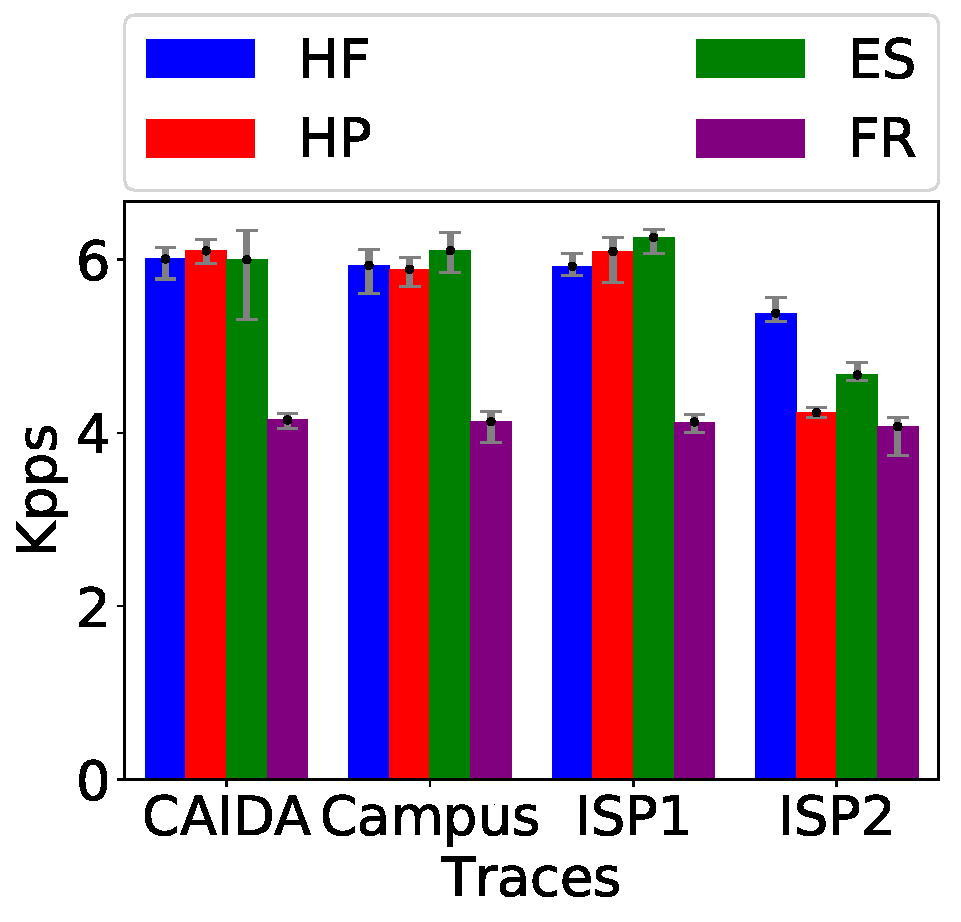
\includegraphics[width=0.9\linewidth]{figures/exp84484/throughput}
%    \caption{The throughput of the algorithms on the four traces.}
%    \label{fig:throughput}
%\end{figure}

%\begin{figure}
%    \centering
%    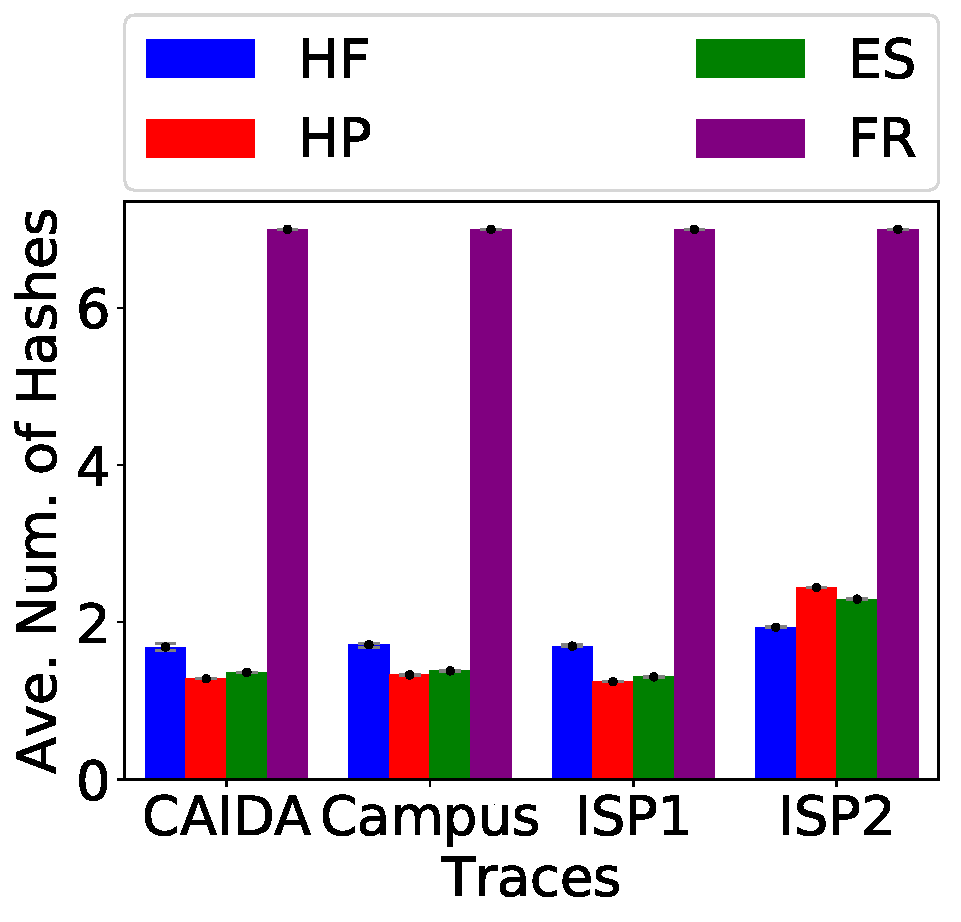
\includegraphics[width=0.9\linewidth]{figures/exp84490/ave_hash}
%    \caption{The average number of hashes for processing a packet.}
%    \label{fig:avehash}
%\end{figure}

%\begin{figure}
%    \centering
%    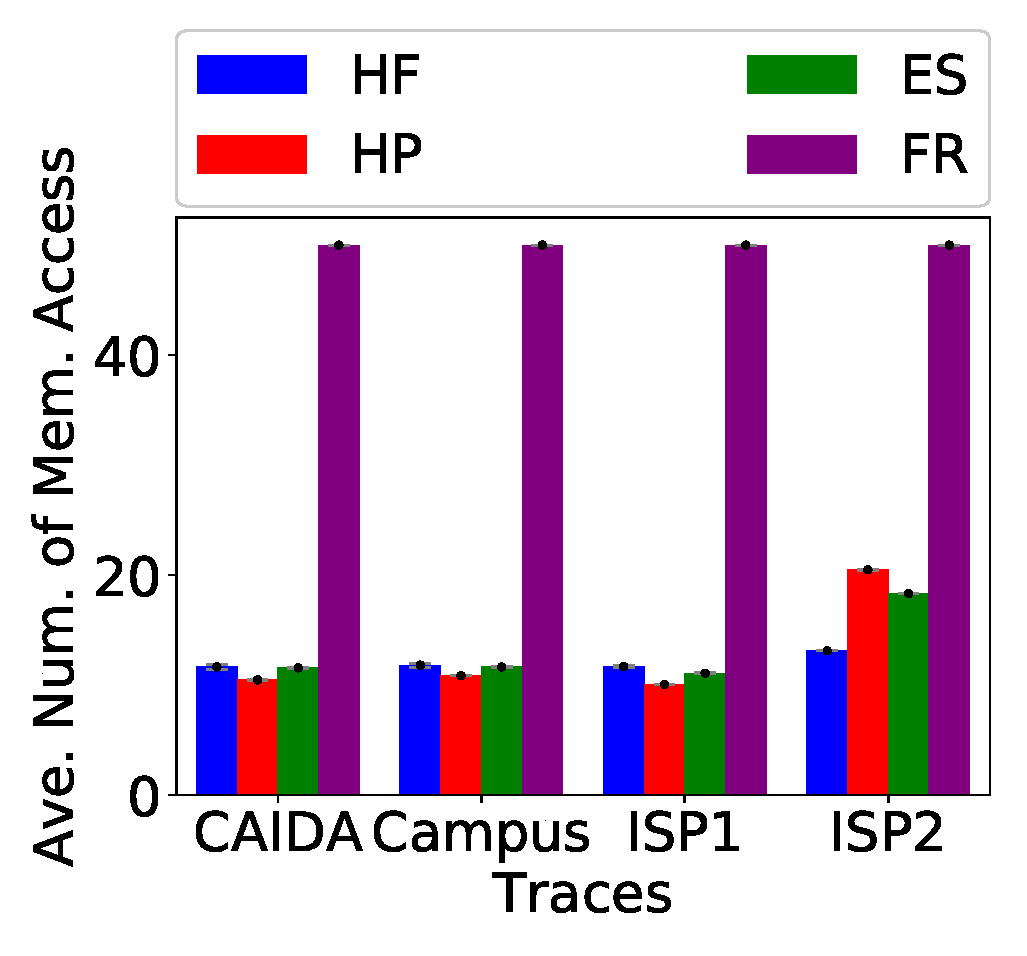
\includegraphics[width=0.9\linewidth]{figures/exp84490/ave_mem}
%    \caption{The average number of memory accesses for processing a packet.}
%    \label{fig:avemem}
%\end{figure}
\fi

%\section{Related Work}
\label{section:relatedwork}
In this section we will present some solutions for network measurement, including the sampling methods as well as the sketches.

The widely adopted method of network measurement in commodity switches/routers are sampling based methods. The basic method of sampling is PS (Packet Sampling), in which the measurement process records a packet for every $M$ packets, or record every packet on the probability of $\frac{1}{M}$. During post processing, the size of the traffic can be gotten by multiplying the number of recorded packets with $M$. However, packet sampling has the drawback of flow size bias, so the elephant flows with far more than $M$ packets are very probably to be recorded, while the mice flows with only a few packets will be missed with high probability. Moreover, we cannot know the specific size of a flow in packet sampling. For example, a flow with only a packet and another flow with more than $M$ packets appears to be the same if only one packet is recorded for each flow. 

PS+SNY\cite{duffield_estimating_2005} proposes that since the majority of the network traffic are the type of TCP and usually each TCP flow corresponds to a SYN packet, we can care about the packets corresponding to the flows with a recorded SYN packet only and discard the packets from the flows without SYN packets. Since each SYN packet is recorded randomly, the flow distribution of the original traffic is the same as the sampled flows with SYN packets. However, this method results in the waste of many packets that don't have a SYN packet associated with them, and the specific size of the flows with SYN packets are not known still. 

Flow Sampling (FS)\cite{hohn_inverting_2003} proposes to select a couple of flows randomly, and once a flow is selected, all the packets corresponding to the flow will be recorded, so we can know the complete information about the recorded flows. Moreover, since the flows are selected randomly, the flow size distribution of the original flows should be the same as the selected flows. However, FS requires to maintain the IDs of the selected flows and query the memory for the selected flows for each incoming packet. So FS is not efficient as PS. 

Dual Sampling (DS)\cite{tune_towards_2008} merges PS and FS by including two components running in parallel, where the first one operates on SYN packets with the sampling probability $p_s$ and the other component operates on non-SYN packets with the sampling probability $p_n$. So DS reduces to PS+SYN when $p_s = p_n$, and approximates to FS when $p_n=1$. 

Since the missing of information is inevitable for the sampling methods, sketches are proposed to record the packets using a compact data structure and fixed computations. 

One of the widely used sketches is count-min sketch\cite{cormode_countmin_2005}. Count-min sketch consists of $d$ rows of counters where each row consists of $r$ counters and has an independent hash function associated with it, which maps a flow ID to a counter of the row. When a packet arrives, it will be mapped to a counter in each row of the sketch, and the corresponding counters will be incremented by 1. On querying the sketch for the size of a particular flow, we will get the counters corresponding to the flow ID in each row and take the minimum one. However, this method requires $2\times d$ memory accesses ($d$ read operations and $d$ write operations) for processing each packet while causing positive bias in flow size estimation.

SCBF\cite{kumar_space-code_2004} is a bit set with $l$ groups of hash functions associated with it. Each group consists of $k$ independent hash functions which map a flow ID to the bit set. When a packet arrives, SCBF randomly chooses a group of the hash functions and map the packet to a group of bits which will be set to 1. When querying for the size of a flow, we get the number of groups of hash functions whose corresponding bits are 1s, which will be used to estimate the size of the flow. MRSCBF is proposed to count the size of very large flows. MRSCBF consists of a group of SCBFs, each of which is associated with a probability $p$. When a packet arrives, a SCBF is updated with the associated probability. The SCBF with small probability will help to estimate the size of large flows. As the algorithm is efficient in memory utilization, it involves too many estimation operations and its precision regarding flow size estimation will be low.

Counter Tree\cite{chen_counter_2017} consists of an array of counters which is organized as a tree of $d$ layers. A counter in the layer-0 and all its ancestors in the higher layers constitute a virtual counter where the counters in the higher layers is the more significant bits of the virtual counter. When a packet arrives, we will hash the packet to a counter in the layer 0 and increment the counter by 1. When the counter at a layer overflows, the parent counter at the next higher layer will be incremented by 1. Finally, counter tree employs statistical tools to remove the noise introduced due to space sharing between different virtual counters.  

SketchVisor\cite{huang_sketchvisor:_2017} aims to bypass the problem of designing efficient sketches. Instead, it designs a fast path which is more efficient in processing packets while less accurate in maintaining information for flows. When the amount of traffic in the network is fair, we can process the packets using a normal sketch, which is more computation intensive but more accurate. When the amount of traffic is greater than a given threshold, we will resort to the fast path to process the overflowing traffic.

The drawback of the sketches is that the accuracy of the maintained information will decrease constantly as the amount of information poured into the sketches increases. In some scenarios it is necessary to maintain only the most important flows and give up the less important flows. ElasticSketch\cite{yang_elastic_2018} and HashPipe\cite{sivaraman_heavy-hitter_2017} introduced in Section~\ref{section:backgroundandmotivation} as well as HashFlow proposed in this paper fall into this category. Another algorithm of this category is HeavyKeeper. 

HeavyKeeper\cite{gong_heavykeeper:_2018} consists of a counting table where each cell contains a flow ID field and a counter field and there is a hash function associated with it. When a packet arrives, the hash function maps the packet to a cell of the counting table by taking the flow ID as input. If collision occurs at the cell, the counter field will be decremented by 1 on the probability of $b^{-C}$, where $b > 1$ and $b \approx 1$, and $C$ is the value of counter field of the cell. The packet's flow ID will be written into the cell and the counter field will be set to 1 if counter field has the value of 0 after decrementing. HeavyKeeper tends to cause negative bias in the flow size estimation of the elephant flows. To minimize the bias it is suggested to create multiple counting tables and take the largest value of the corresponding cells' counters from each counting table as the estimated flow size, which will be inefficient in utilization of memory.

\section{Conclusion}
\label{section:conclusion}
We propose HashFlow for efficient collection of flow records, 
which is useful for a wide range of measurement and analysis applications. 
The collision resolution and record promotion strategy is of central importance 
to HashFlow's accuracy and efficiency. We analyze the performance bound 
of HashFlow based on a probabilistic model, and implement it in a software switch as well as a hardware switch. 
The evaluation results based on real traces from different networks show that, 
HashFlow consistently achieves a clearly better performance in nearly all cases. 
In the future, we plan to study how to make it adaptive to more accurate measurement of mice flows and network wide measurement.

\section{Acknowledgement}
\label{section:acknowledgement}
We thank the anonymous ICDCS reviewers for their valuable comments. This work is supported by the National Natural Science Foundation of China(Grant No. 61702315) and PCL Future Regional Network Facilities for Large-scale Experiments and Applications (PCL2018KP001).
\bibliographystyle{IEEEtran}
%\bibliographystyle{havard}
\bibliography{ms}
\end{document}